\documentclass[12pt, a4paper, oneside]{ctexart}

\title{\kaishu\fontsize{22pt}{22pt}\selectfont 《面向对象程序设计》课程设计进度报告}
\date{}

\usepackage{graphicx}
\usepackage{listings}
\usepackage{xcolor}
\usepackage{float} % 导言区添加
\usepackage{caption} % 添加这一行
\lstset{
  breaklines=true,             % 代码过长时自动换行
  columns=flexible,            % 让空格和中文显示更自然,防止对齐错乱
  basicstyle=\ttfamily,        % 代码使用等宽字体
  keywordstyle=\color{blue},   % 关键字高亮为蓝色
  commentstyle=\color{gray},   % 注释高亮为灰色
  stringstyle=\color{red},     % 字符串高亮为红色
  showstringspaces=false,      % 不显示字符串中的空格符号
  numbers=left,                % 在左侧显示行号
  numberstyle=\tiny,           % 行号使用小号字体
}

\begin{document}

% 标题
\maketitle

% logo
\vspace{-6em}  % 减少与标题的间距
\centering

\includegraphics[width=0.3\textwidth]{../images/湖南理工学院logo..png}

% 基本信息
\begin{flushleft}
\songti\fontsize{18pt}{18pt}\selectfont 课程设计题目:八皇后问题

\vspace{1em}
\songti\fontsize{18pt}{18pt}\selectfont \hspace{2em}专业班级:********

\vspace{1em}
\songti\fontsize{18pt}{18pt}\selectfont \hspace{2em}小组成员:\hspace{0.5em}姓名\hspace{4em}学号\hspace{3.5em}序号

\vspace{1em}
\songti\fontsize{18pt}{18pt}\selectfont \hspace{7em}******\hspace{2em}***********\hspace{2.5em}1

\vspace{1em}
\songti\fontsize{18pt}{18pt}\selectfont \hspace{7em}******\hspace{2em}***********\hspace{2.5em}2

\vspace{1em}
\songti\fontsize{18pt}{18pt}\selectfont \hspace{7em}******\hspace{2em}***********\hspace{2.5em}3

\vspace{1em}
\songti\fontsize{18pt}{18pt}\selectfont \hspace{7em}******\hspace{2em}***********\hspace{2.5em}4

\vspace{1em}
\songti\fontsize{18pt}{18pt}\selectfont 设计时间:2025-06-10 \hspace{4em}批阅时间:

\vspace{1em}
\songti\fontsize{18pt}{18pt}\selectfont 指导教师:****** \hspace{7em} 成绩:

\vspace{1em}
\songti\fontsize{18pt}{18pt}\selectfont 自评等级:良
\end{flushleft}

\newpage % 新的一页

% 目录
\clearpage
\tableofcontents
\clearpage

\newpage % 新的一页

% 正文

\section{设计题目}
\begin{flushleft}
\songti\fontsize{16pt}{16pt}\selectfont
八皇后问题(三法实现)
\end{flushleft}

\section{实验目的}
\begin{flushleft}
\songti\fontsize{16pt}{16pt}\selectfont
1.  理解八皇后问题的基本概念及其约束条件。

2.  掌握回溯法的基本思路,并实现递归回溯、非递归回溯和排列树回溯三种算法。

3.  对比三种算法的效率,分析其优缺点。
\end{flushleft}

\section{实验环境}
\begin{flushleft}
\songti\fontsize{16pt}{16pt}\selectfont
操作系统:Windows 11

开发环境:CLion IDE 2025.1.2

编程语言:C++

编译选项:C++20,MSVC 2022
\end{flushleft}

\section{实验内容}

\subsection{内容描述}
\begin{flushleft}
\songti\fontsize{16pt}{16pt}\selectfont
在一个8×8的国际象棋棋盘上放置8个皇后,要求每个皇后两两之间不相“冲突”(在每一横列,竖列,斜列只有一个皇后)。
\end{flushleft}

\subsection{项目要求}
\begin{flushleft}
\songti\fontsize{16pt}{16pt}\selectfont
(1)使用非递归回溯,递归回溯,排列树的递归回溯实现。

(2)找出所有的解。

(3)设计相应的选择界面。
\end{flushleft}

\subsection{算法实现}
\begin{flushleft}
\songti\fontsize{16pt}{16pt}\selectfont
(1)递归回溯法

基本思路:逐位置放置皇后,检查是否冲突,若不冲突则递归处理下一行,否则回溯。

核心代码:
\end{flushleft}

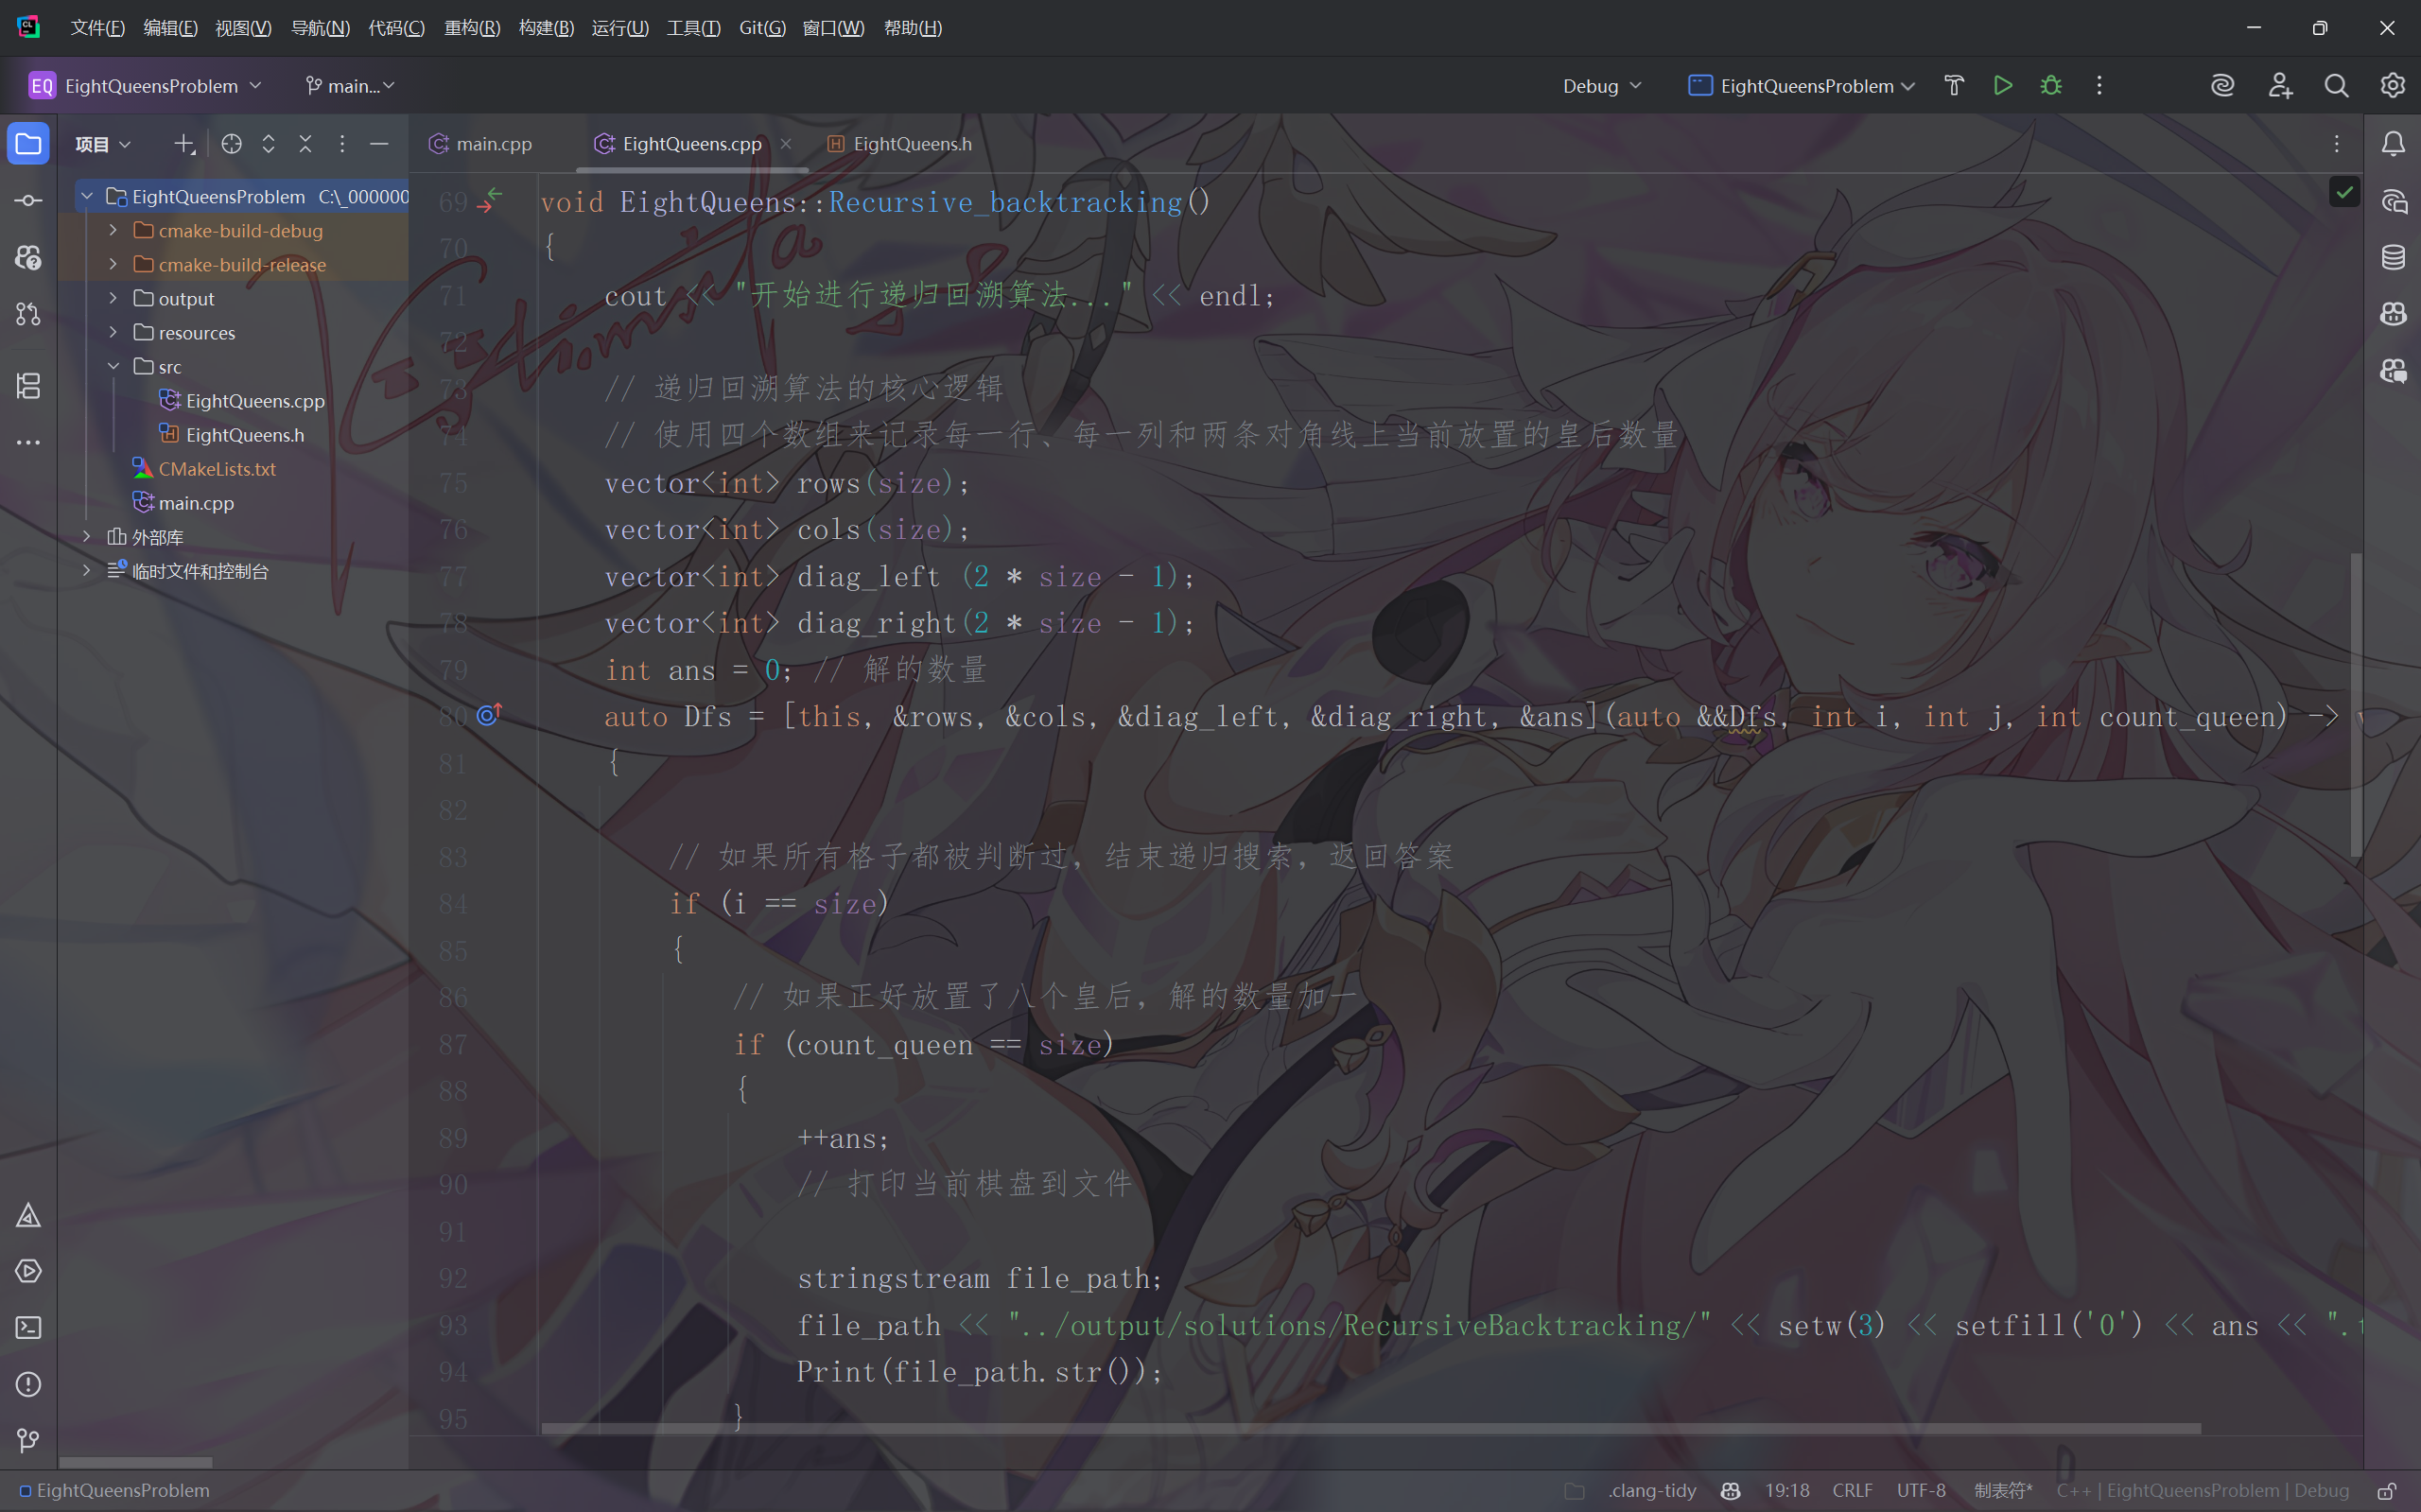
\includegraphics[width=\textwidth]{../images/递归回溯代码1.png}\\[0.5em]
\captionof{figure}{递归回溯代码1}
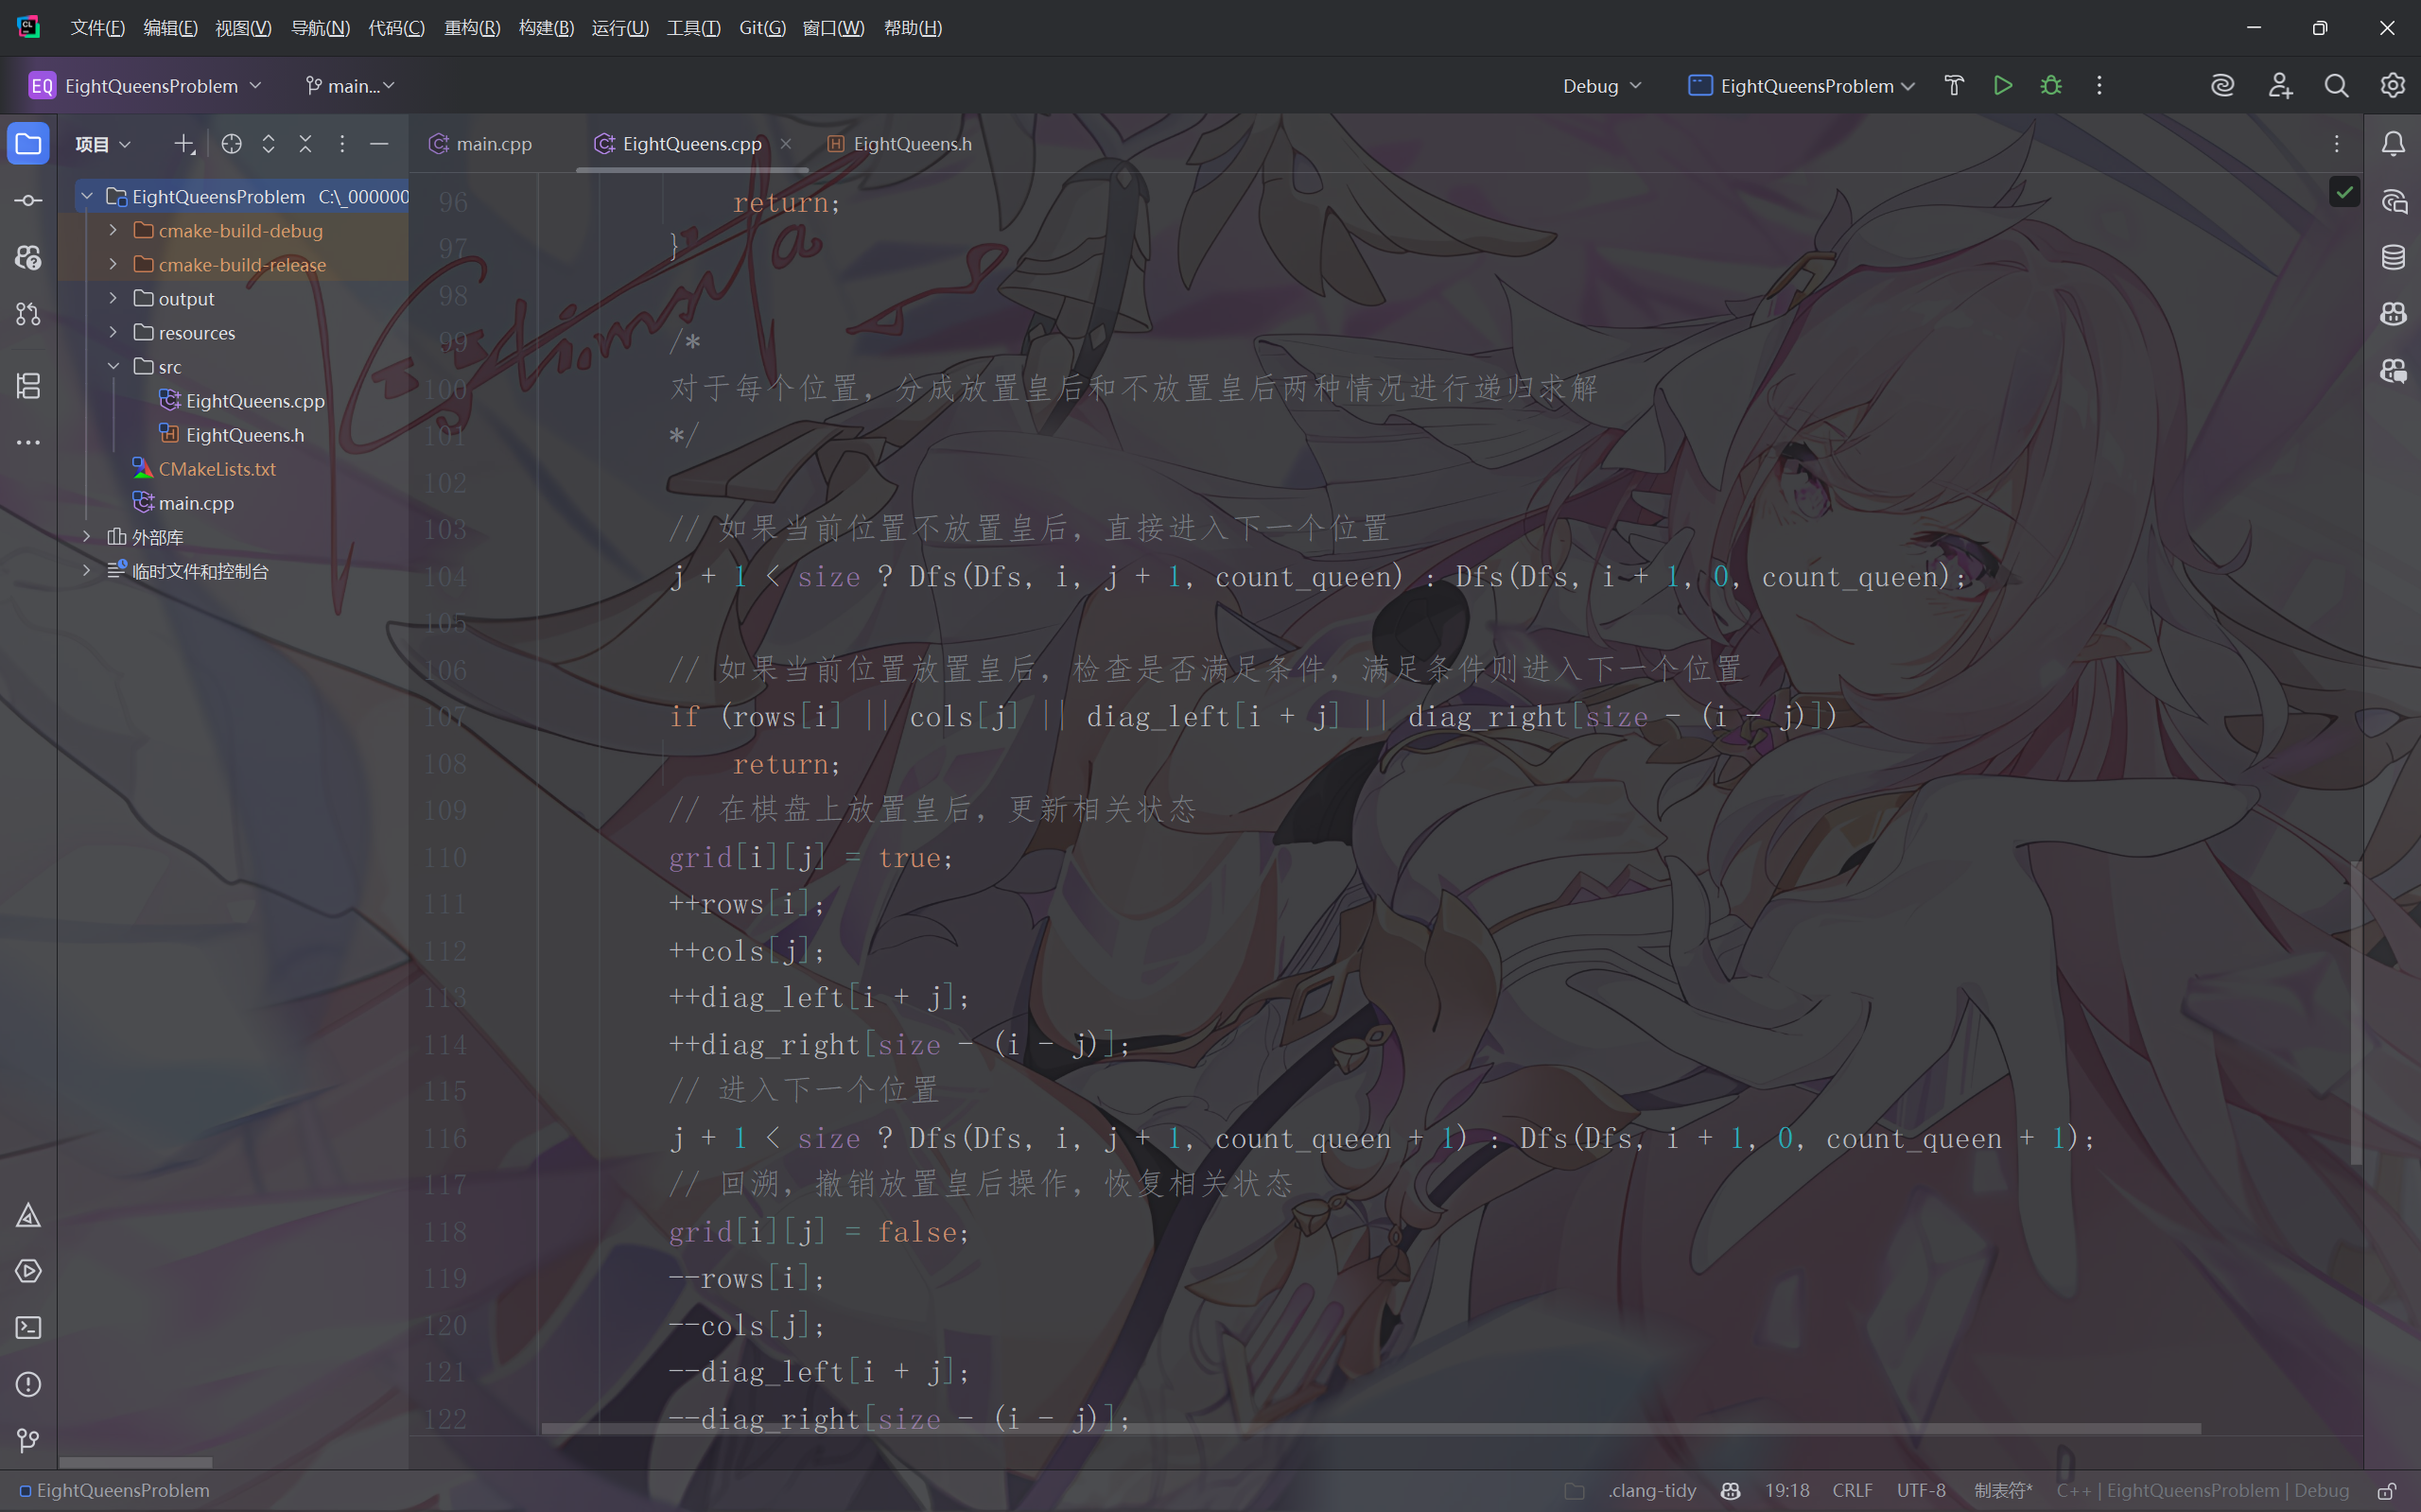
\includegraphics[width=\textwidth]{../images/递归回溯代码2.png}\\[0.5em]
\captionof{figure}{递归回溯代码2}
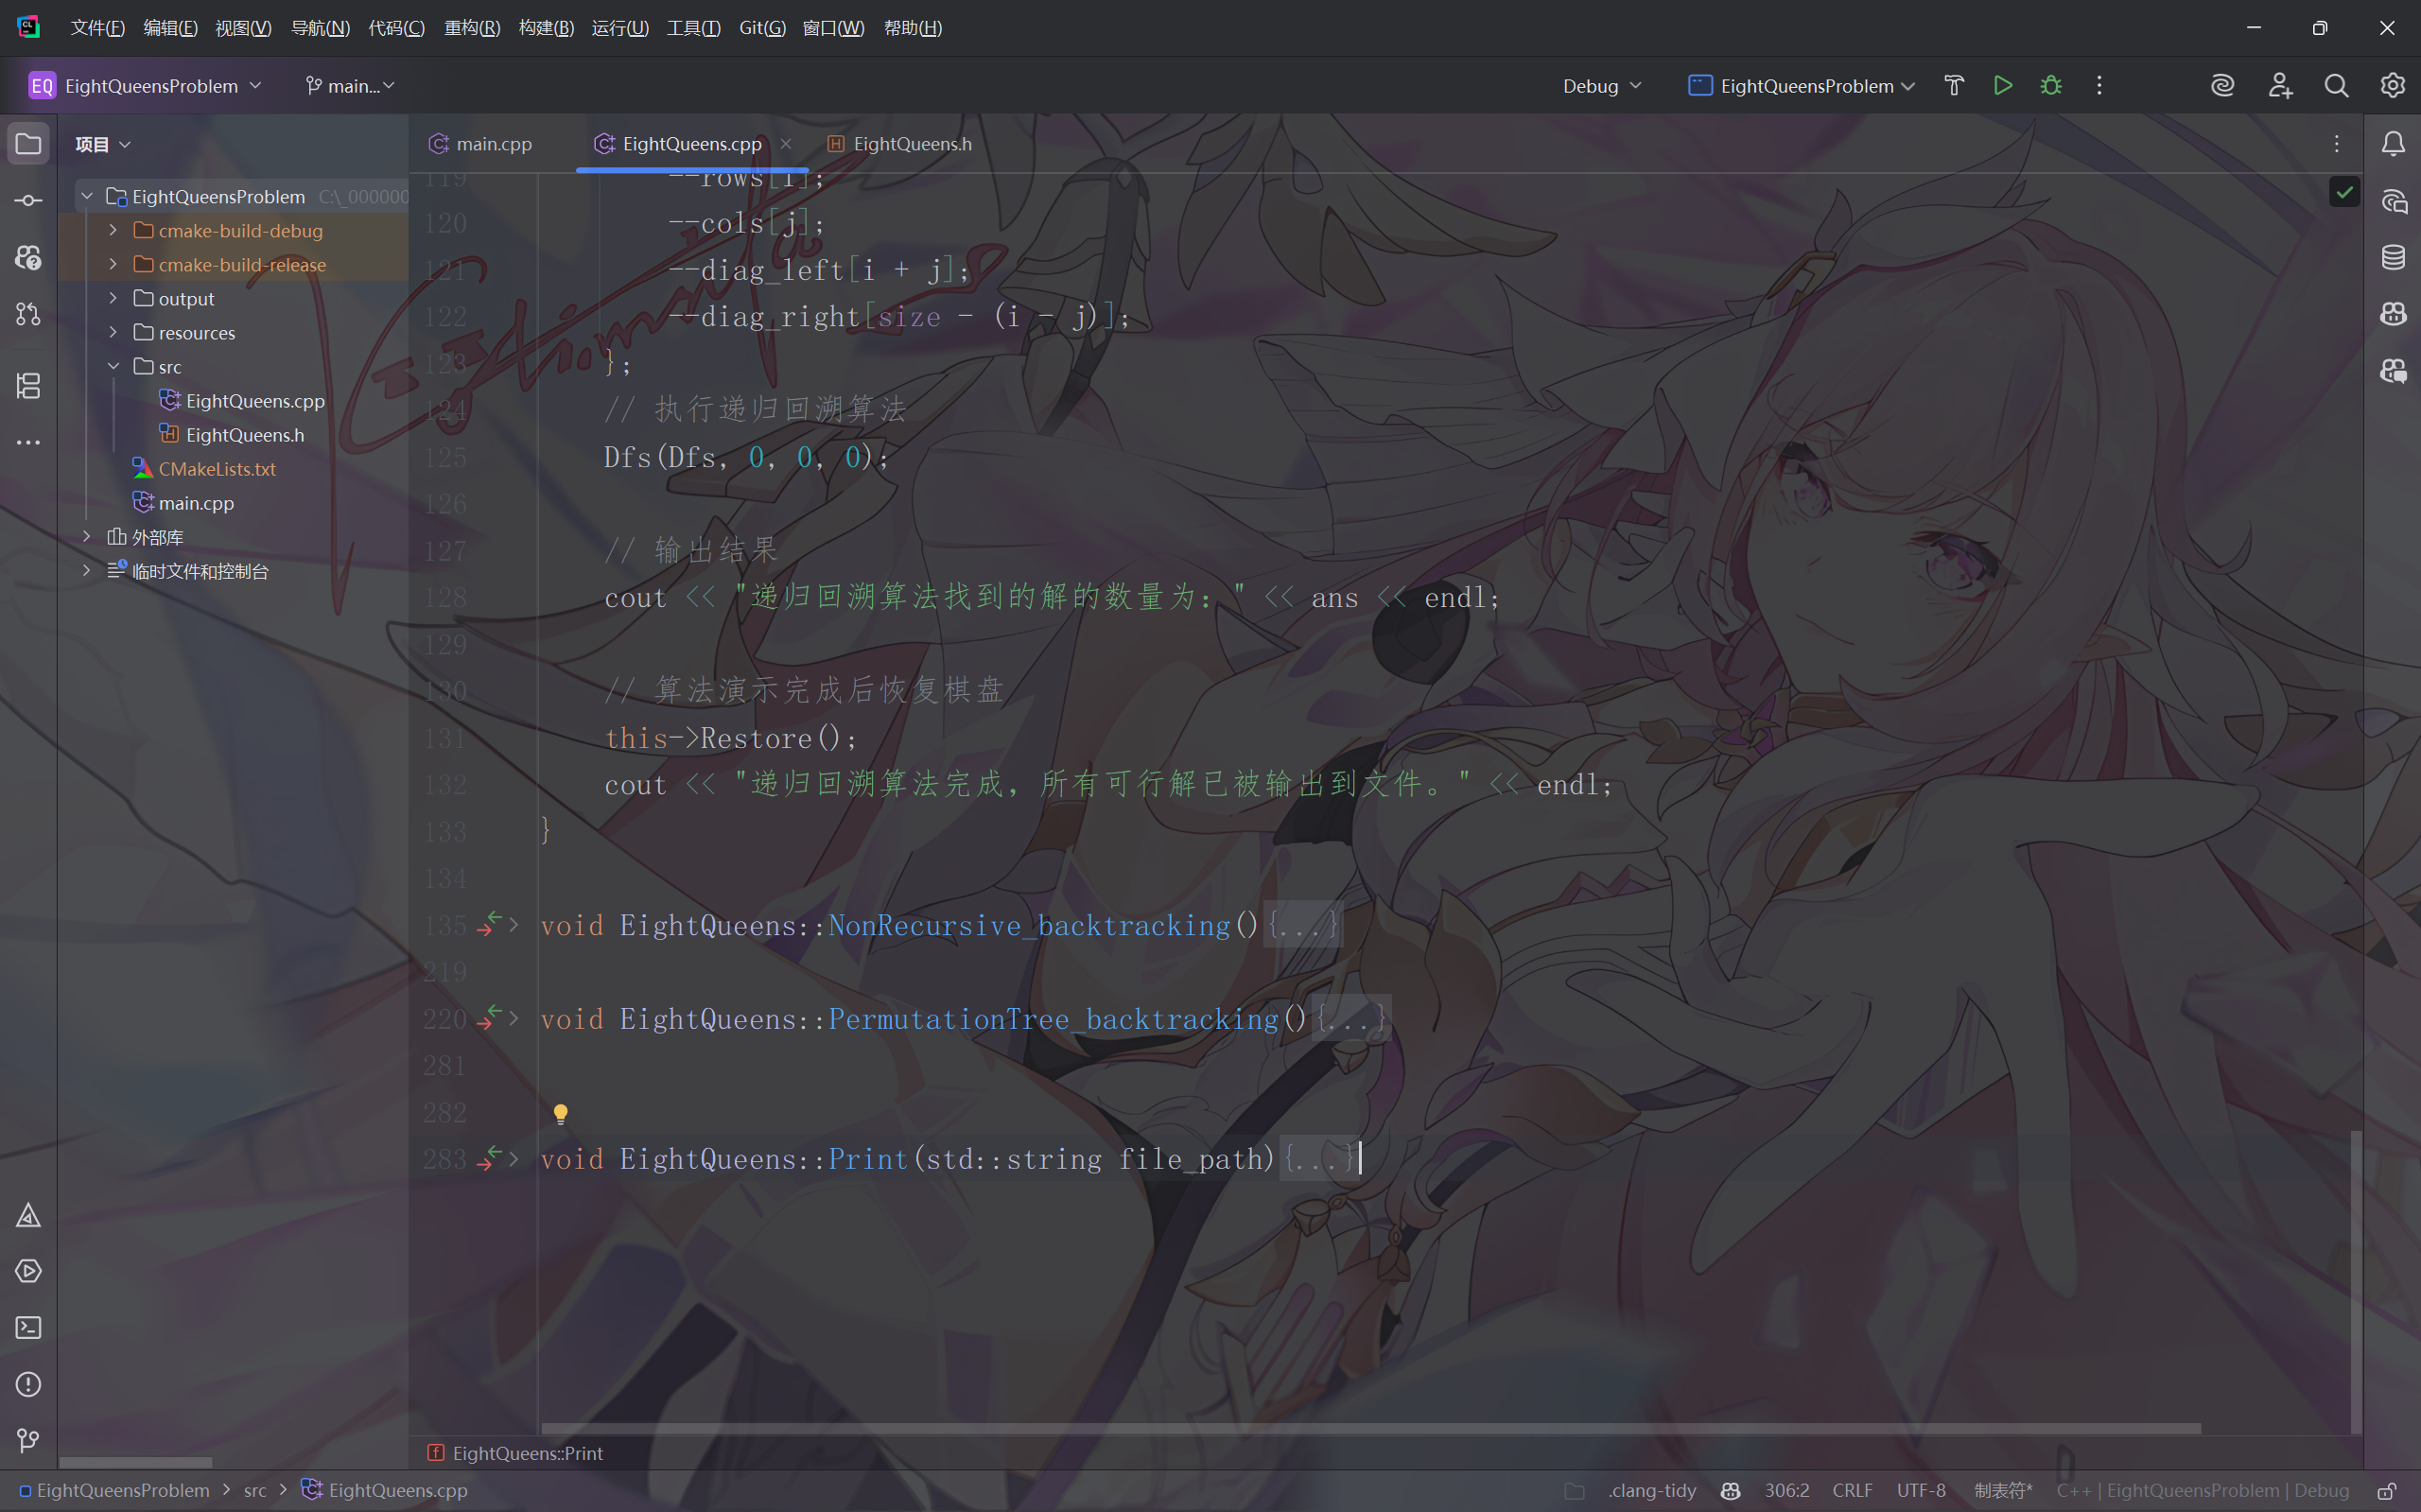
\includegraphics[width=\textwidth]{../images/递归回溯代码3.png}\\[0.5em]
\captionof{figure}{递归回溯代码3}

\begin{flushleft}
\songti\fontsize{16pt}{16pt}\selectfont
(2)非递归回溯法

基本思路:用循环和栈模拟递归过程,避免函数调用开销。

核心代码:
\end{flushleft}

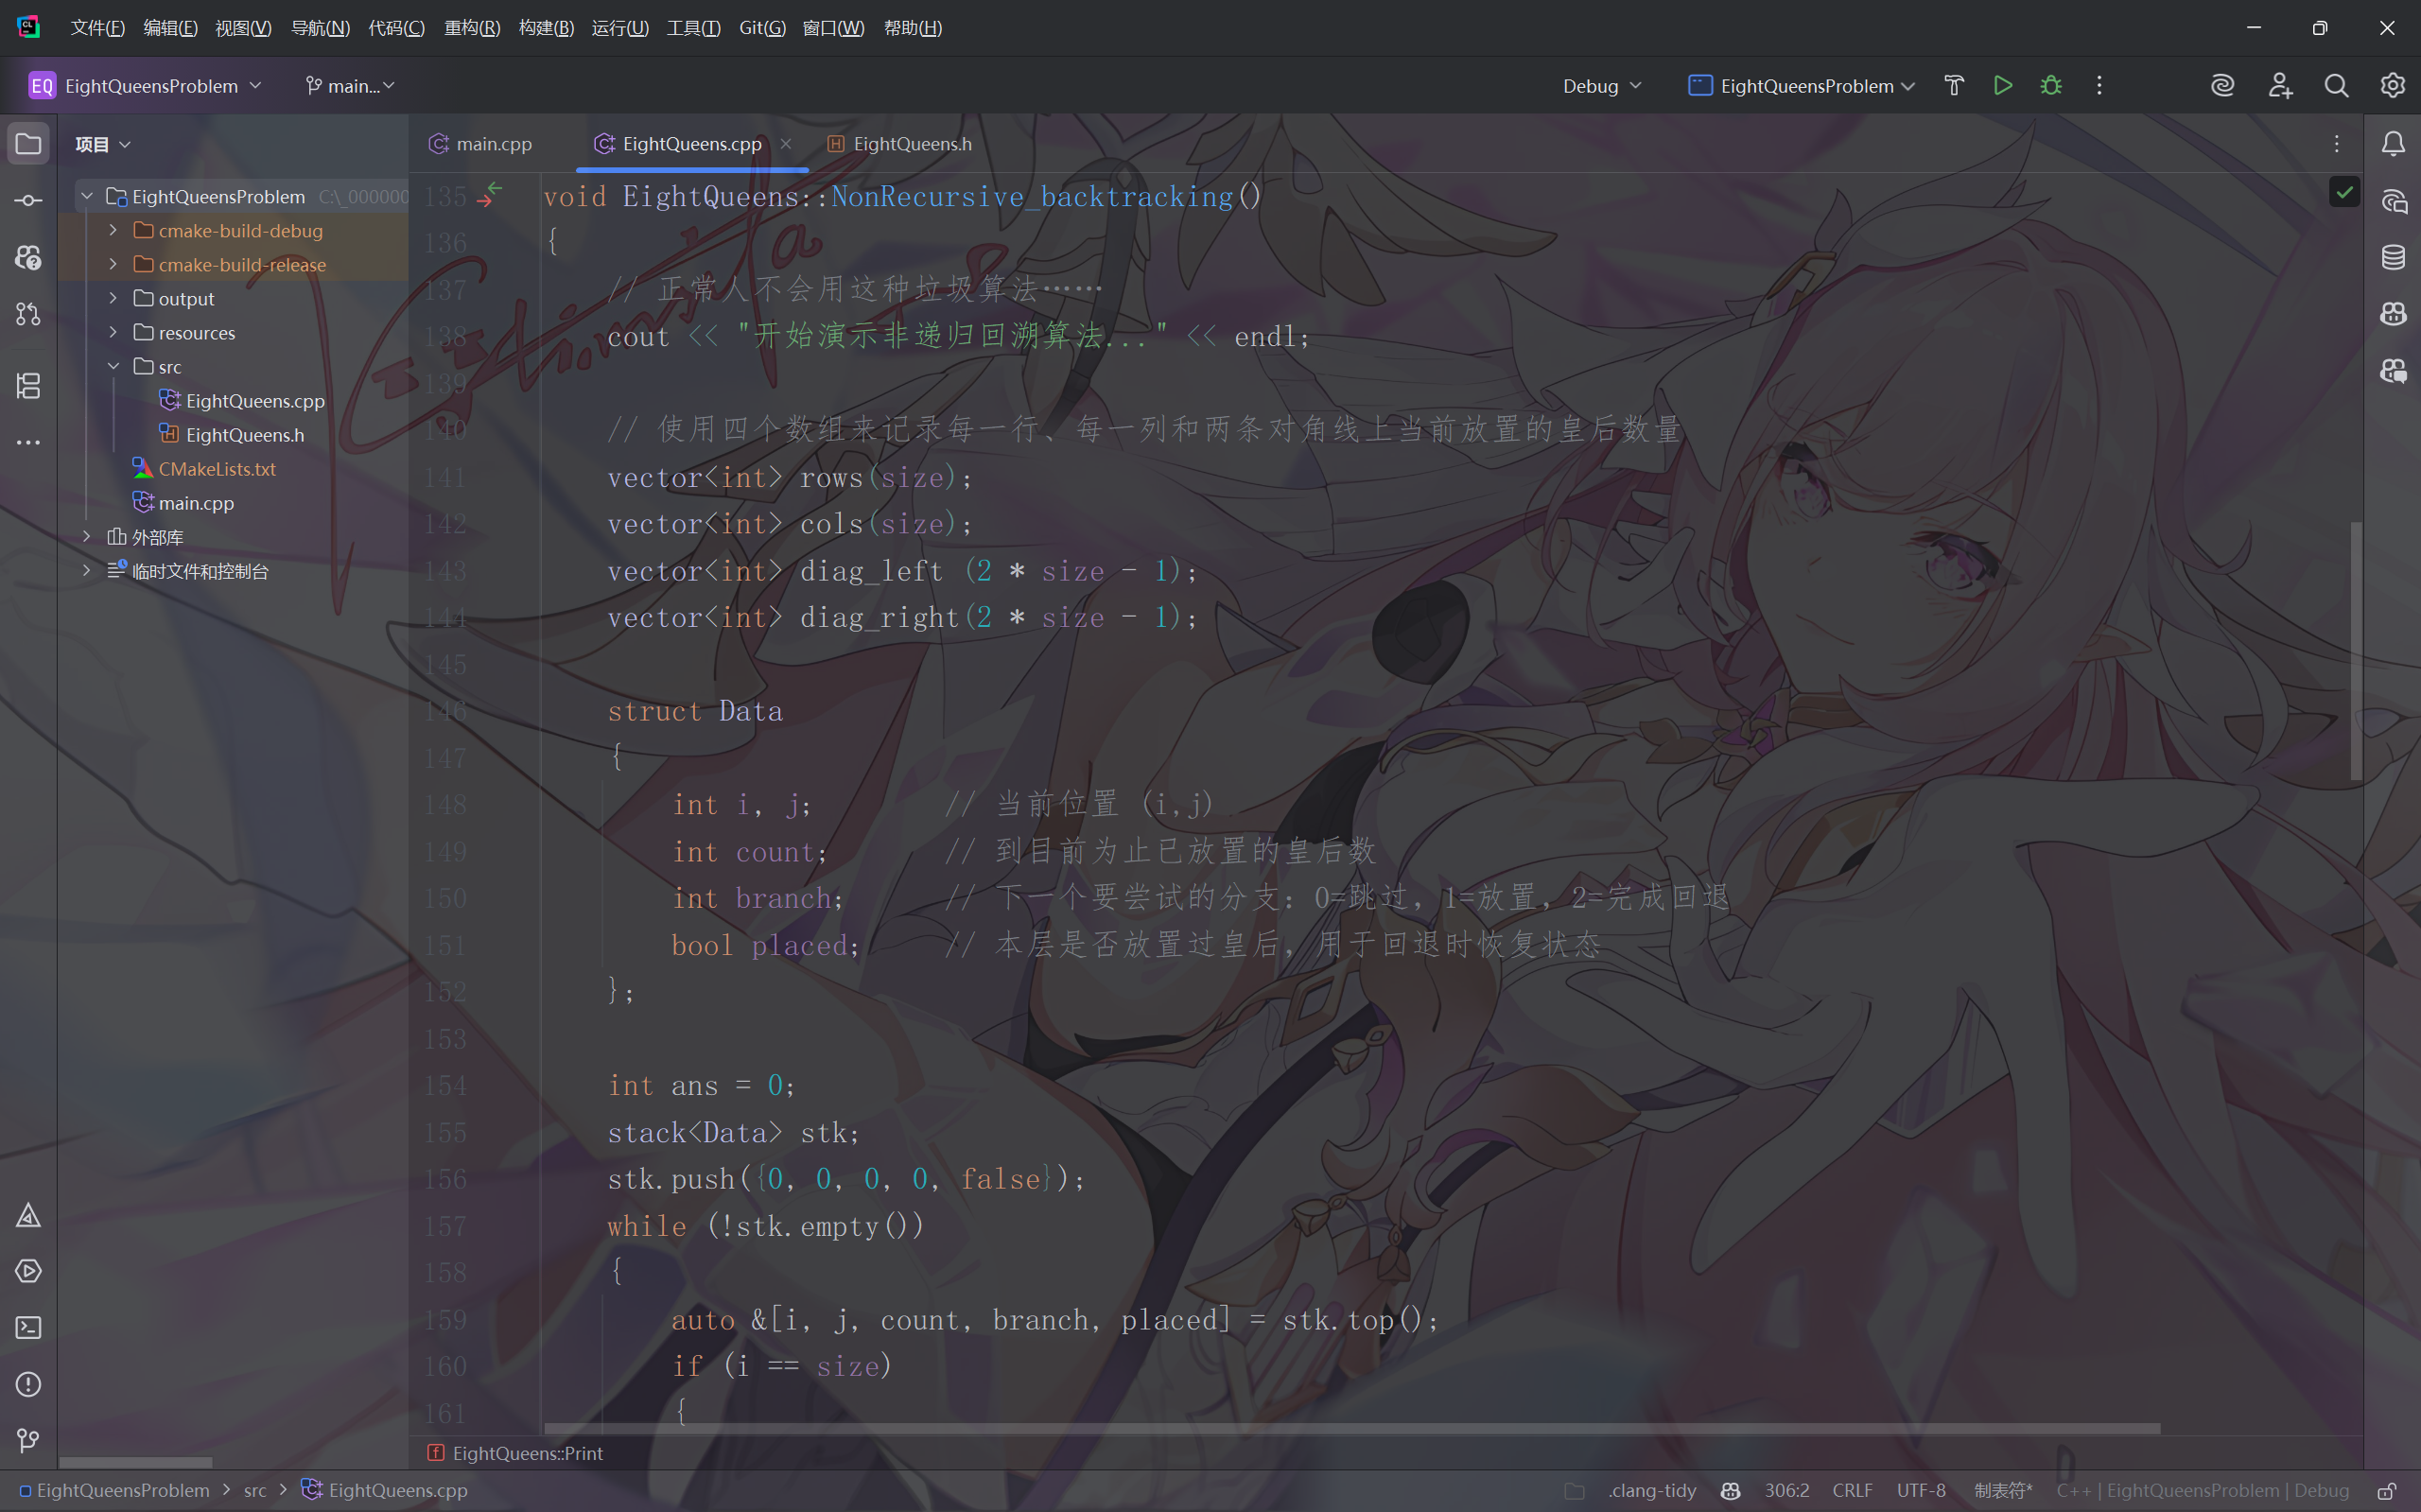
\includegraphics[width=\textwidth]{../images/非递归回溯代码1.png}\\[0.5em]
\captionof{figure}{非递归回溯代码1}
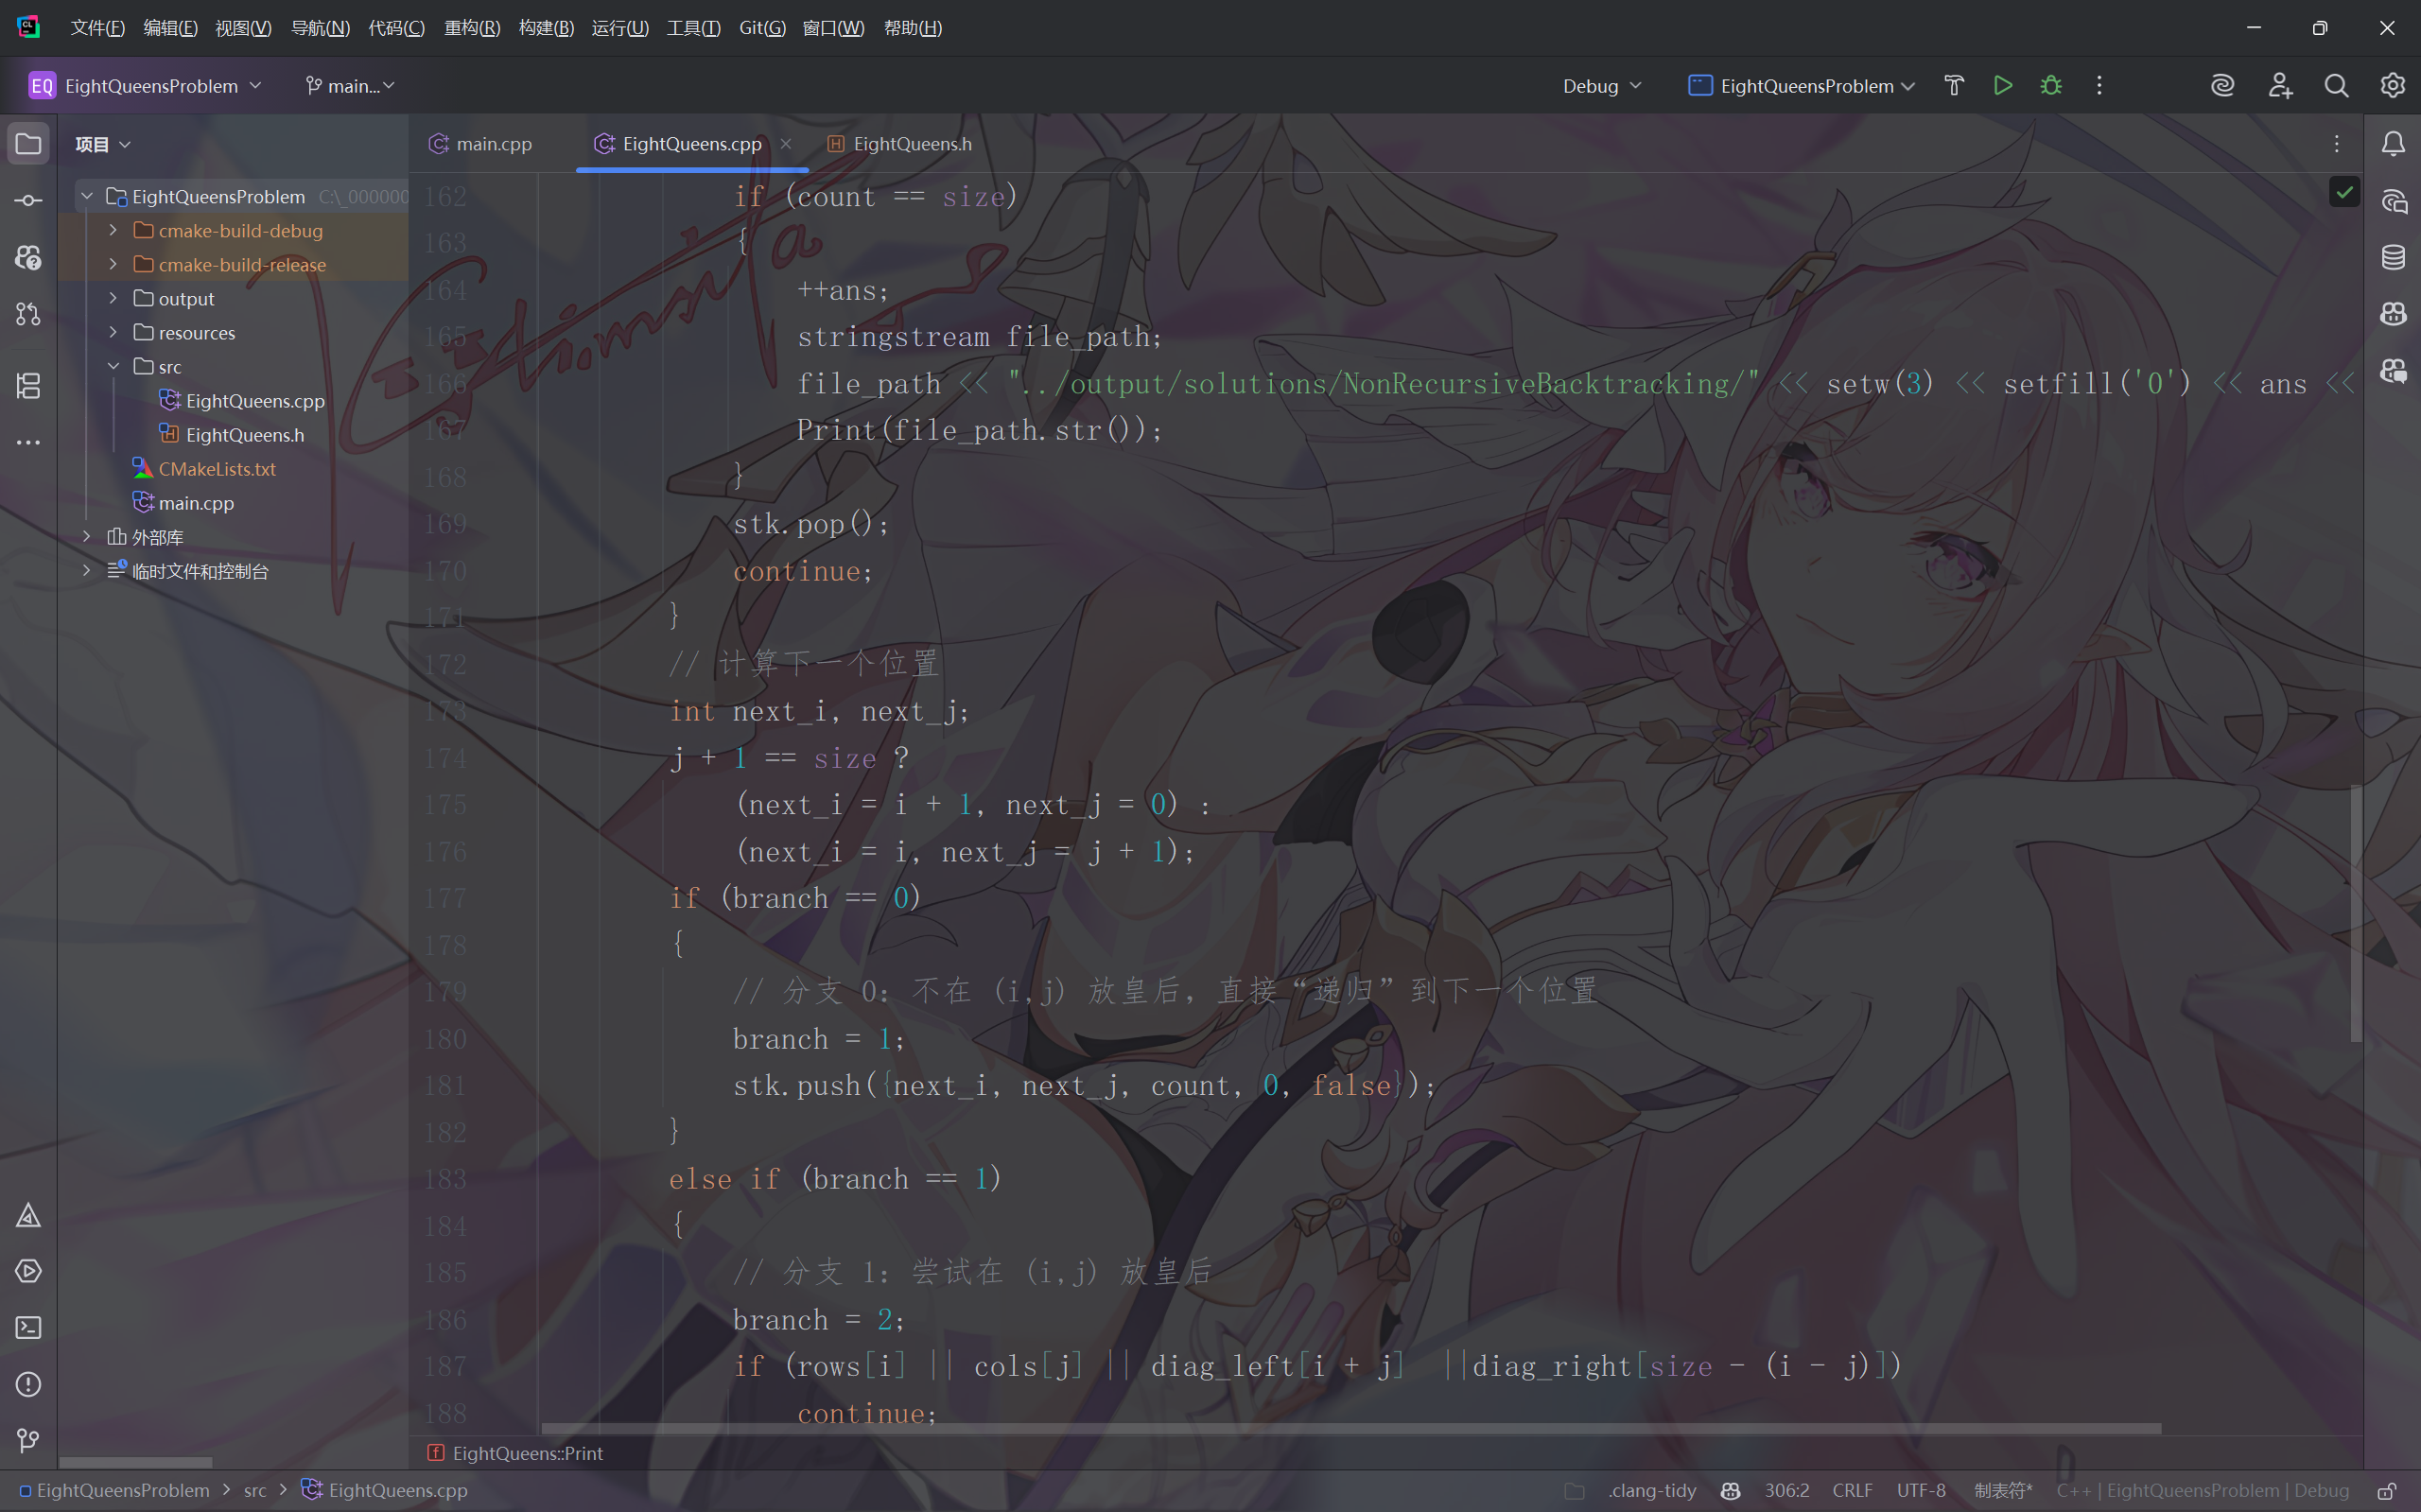
\includegraphics[width=\textwidth]{../images/非递归回溯代码2.png}\\[0.5em]
\captionof{figure}{非递归回溯代码2}
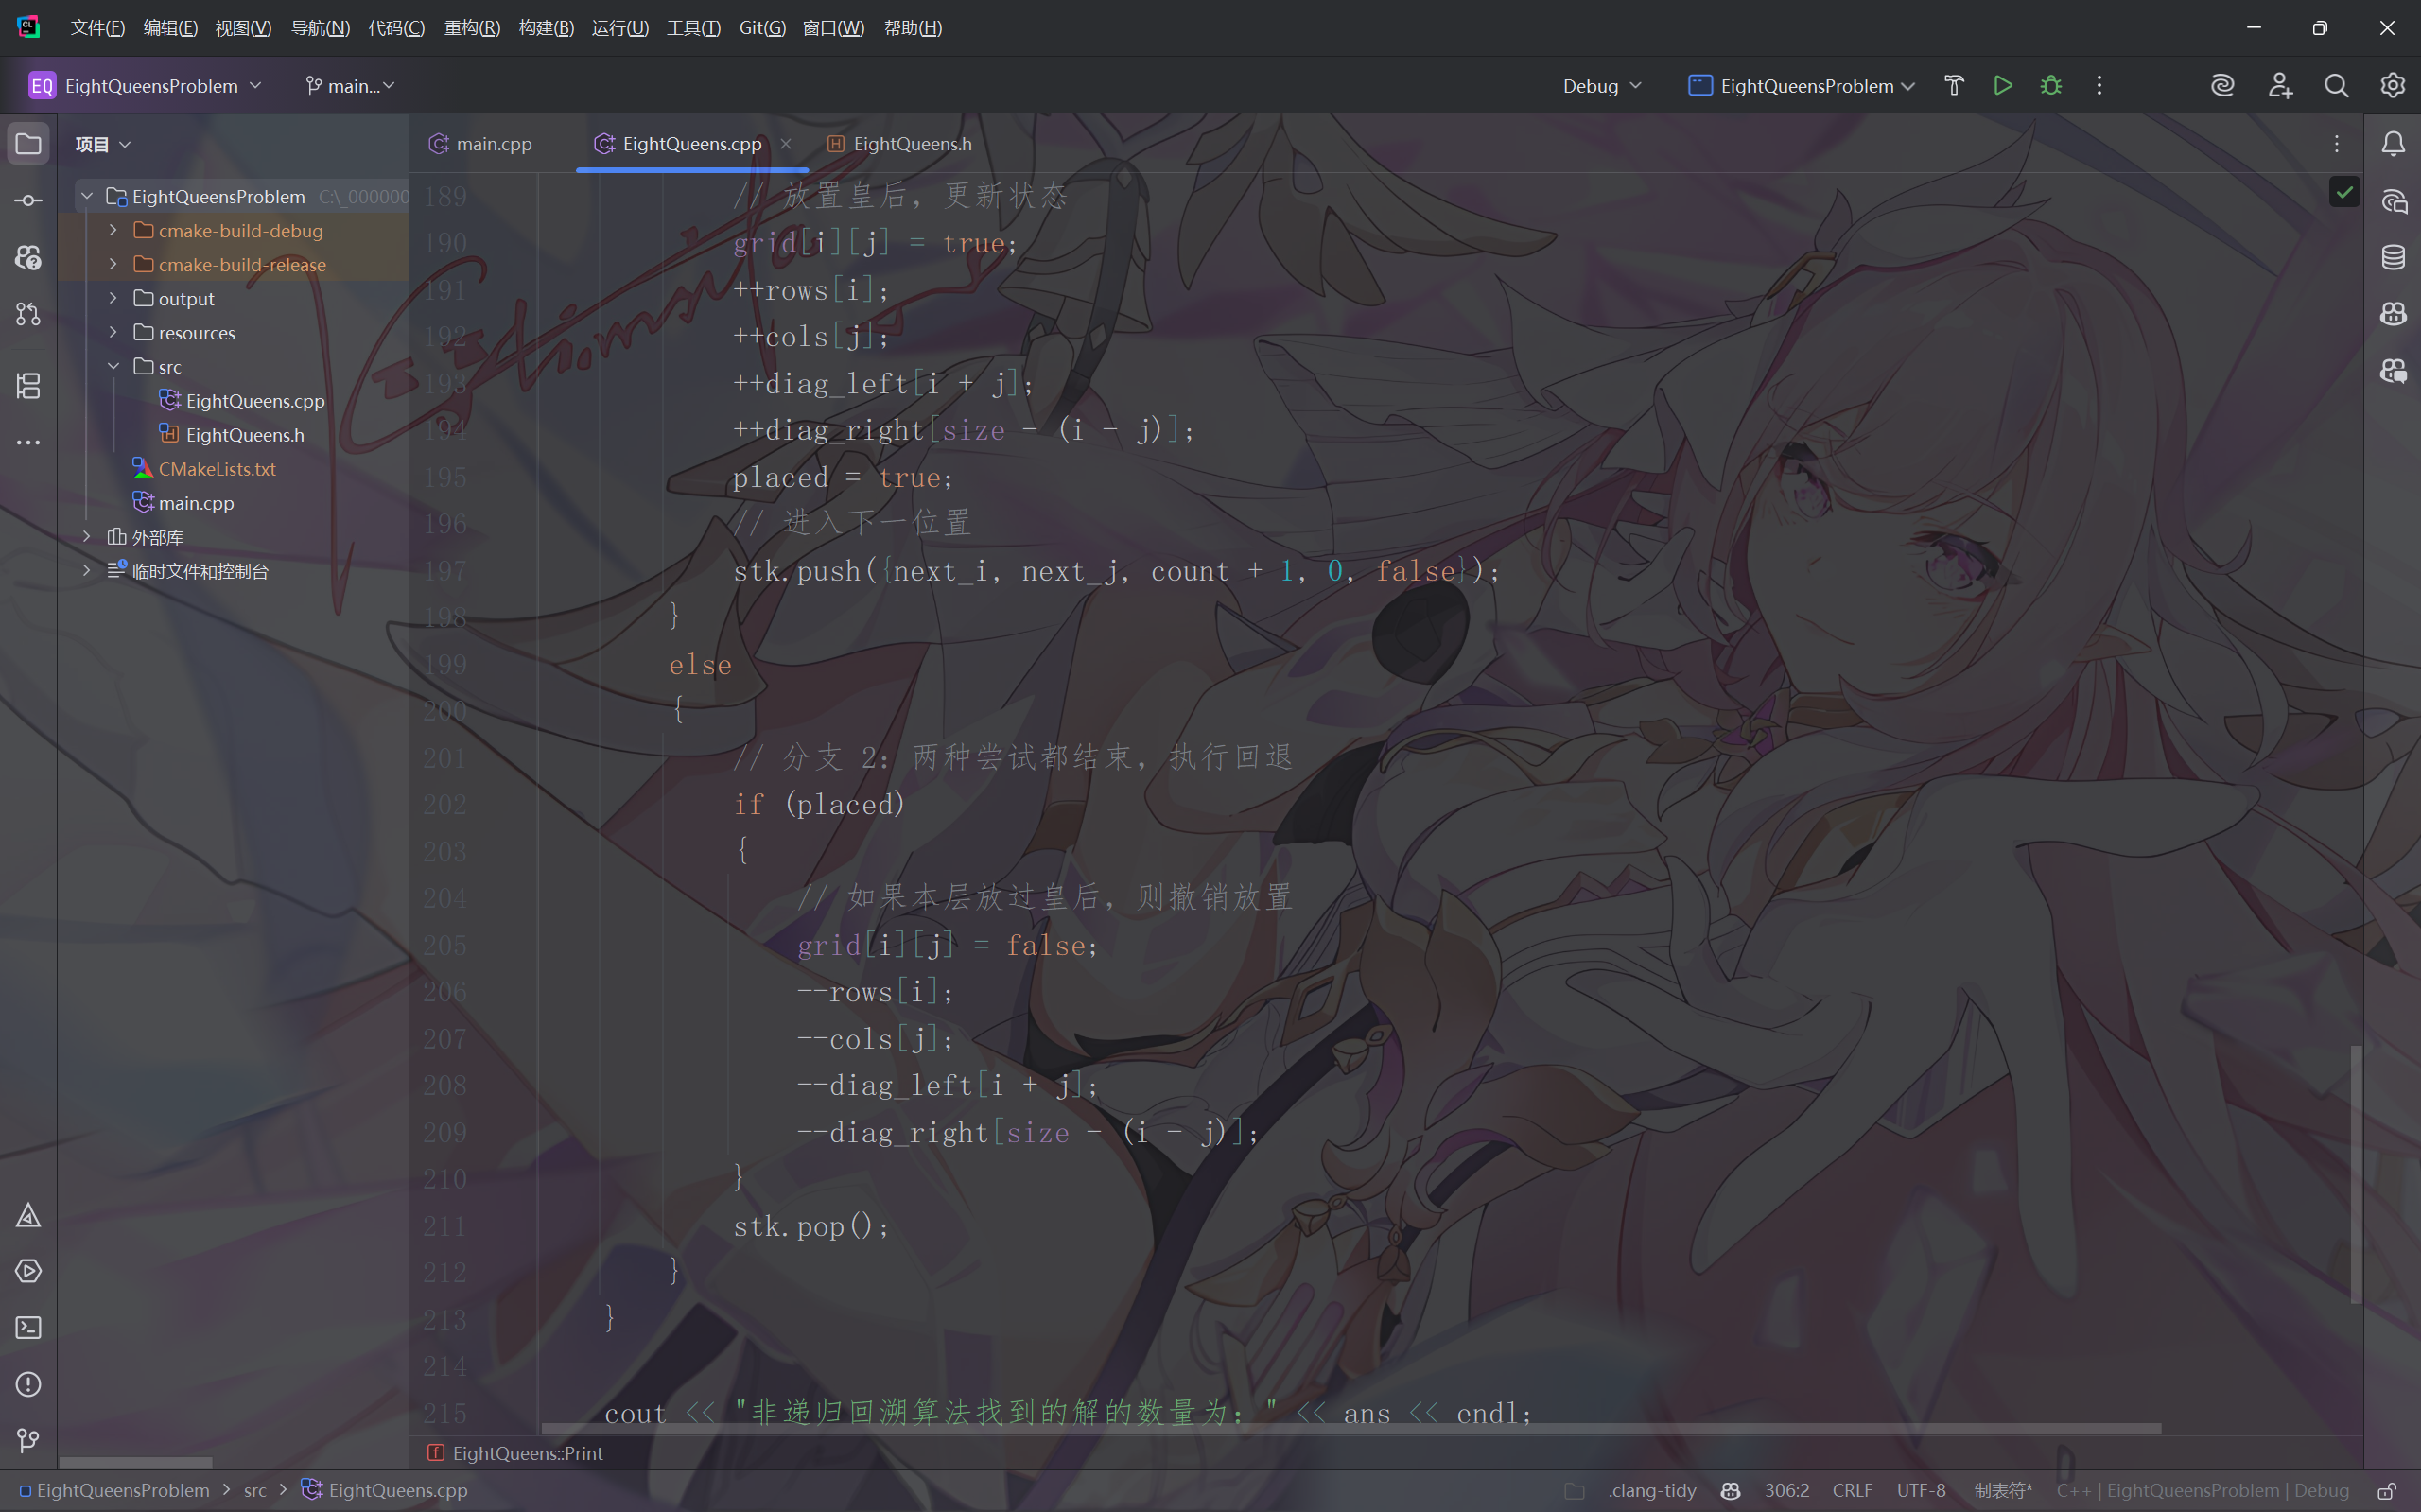
\includegraphics[width=\textwidth]{../images/非递归回溯代码3.png}\\[0.5em]
\captionof{figure}{非递归回溯代码3}
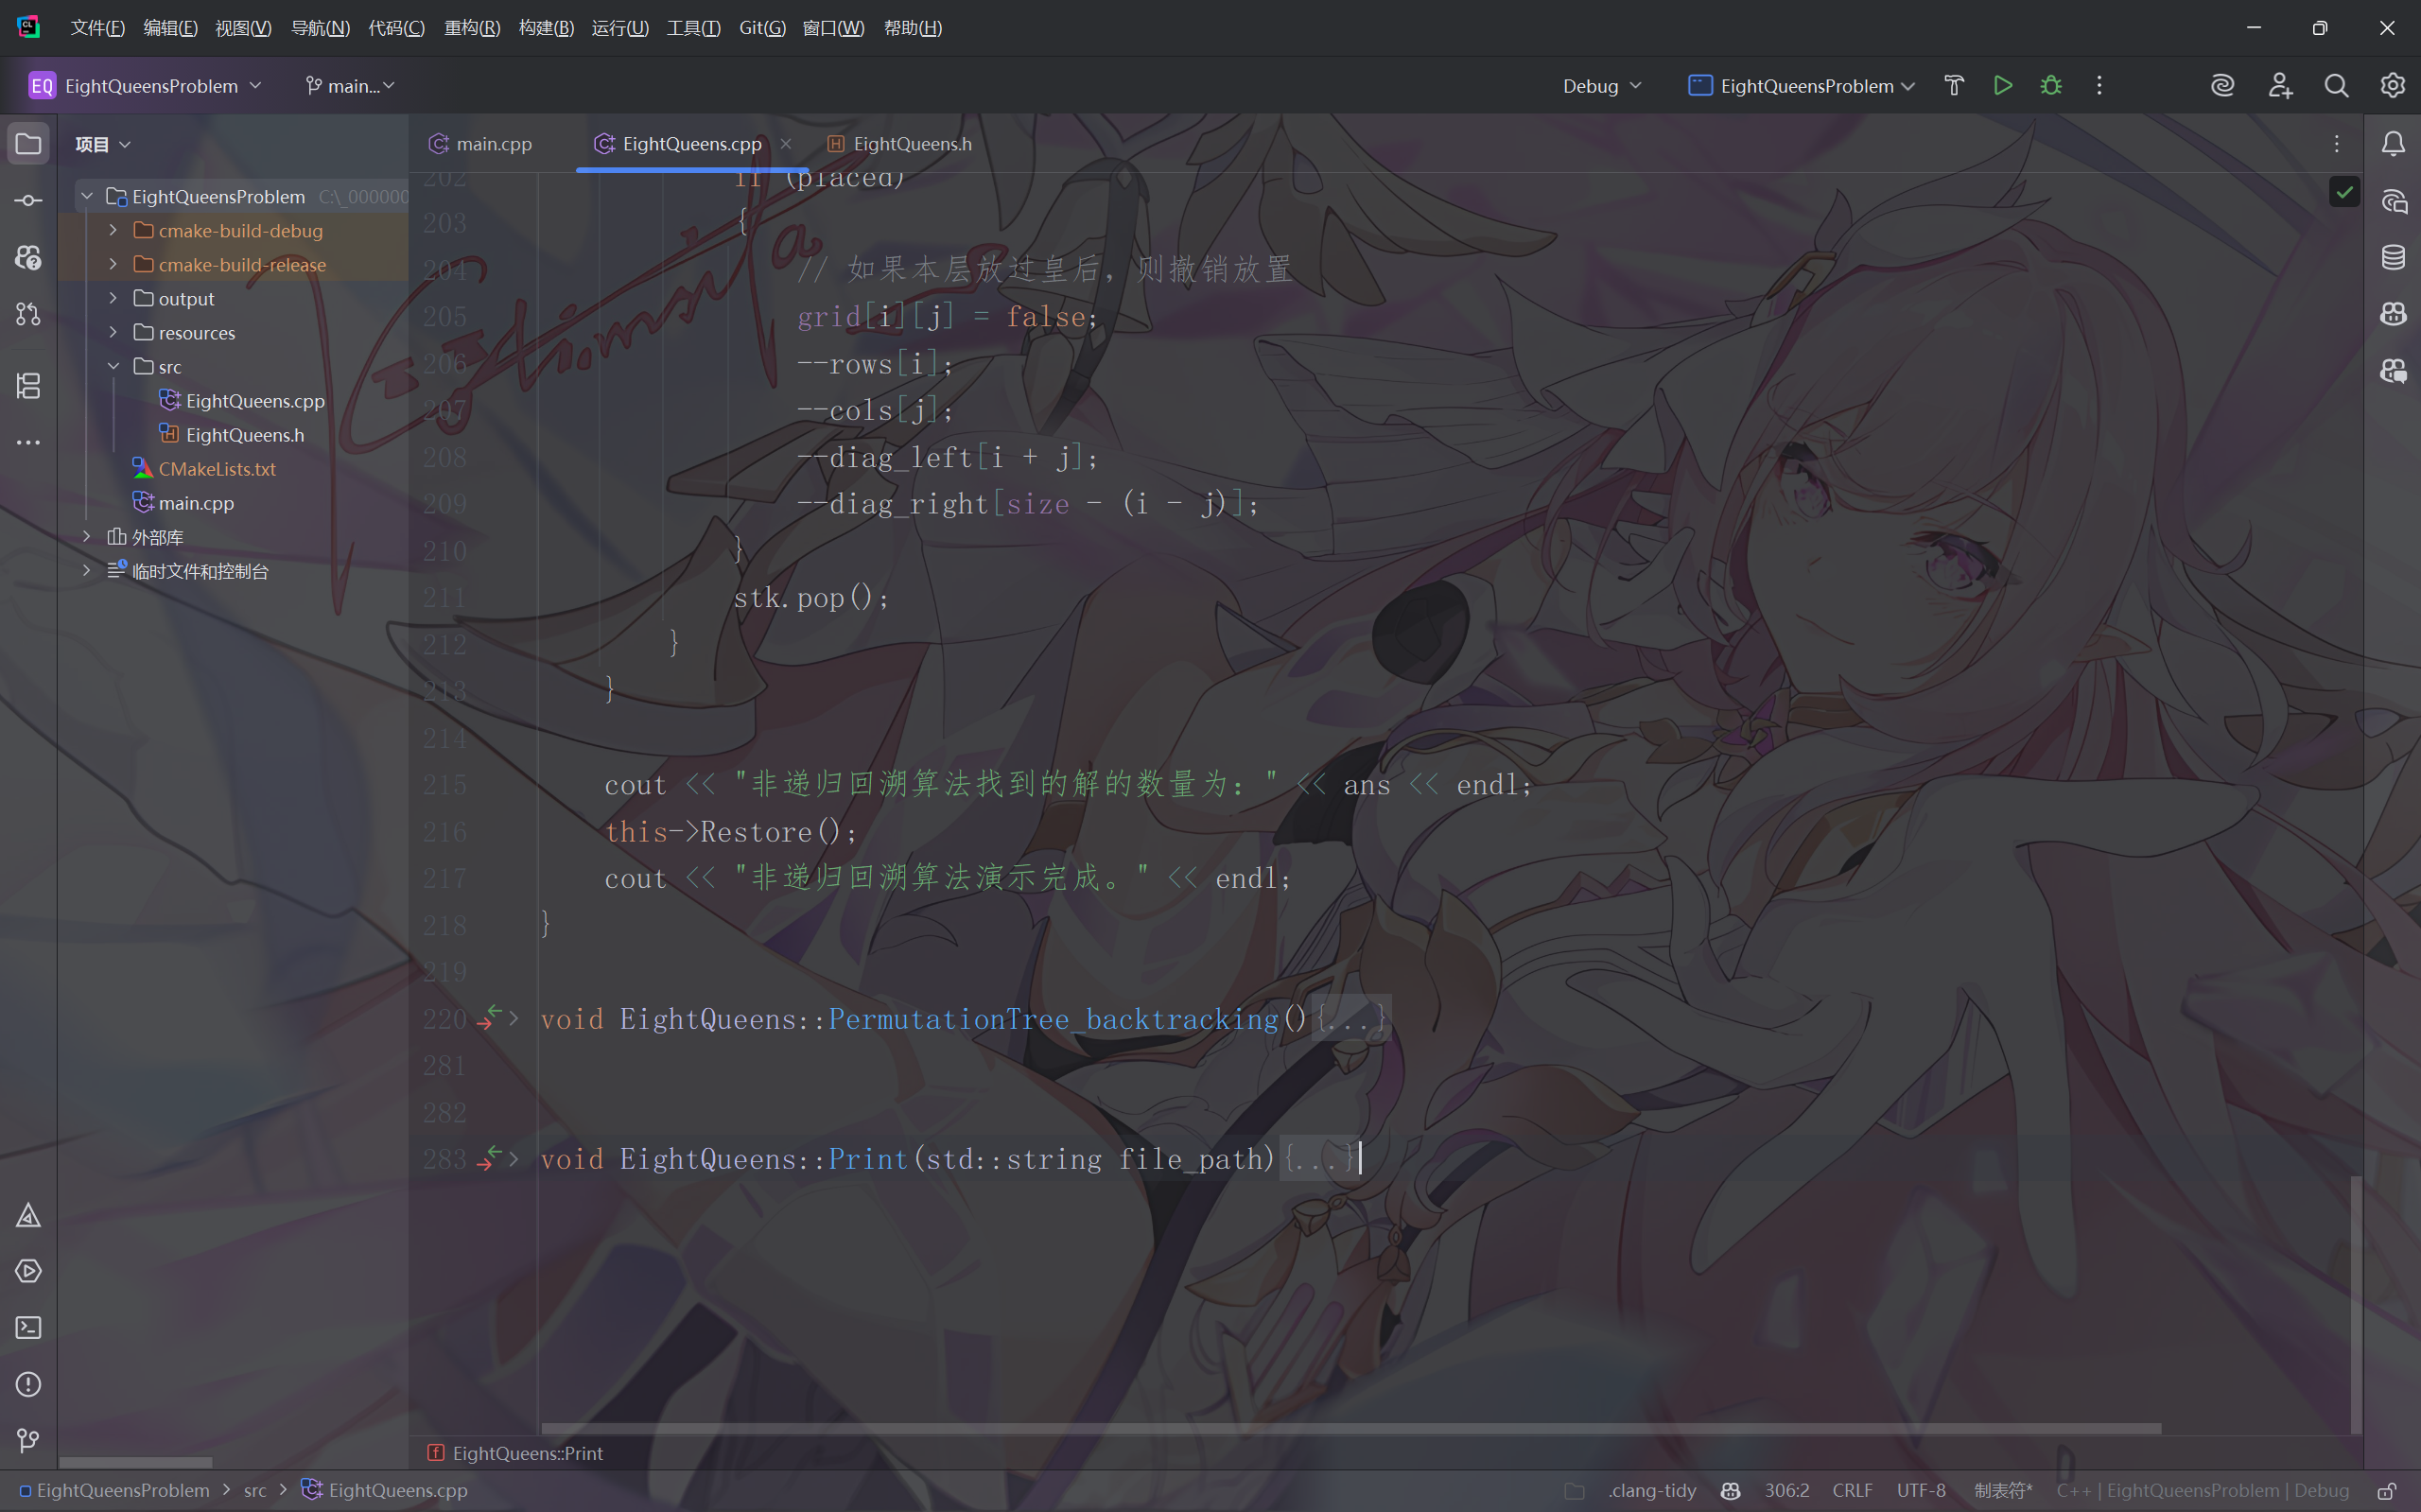
\includegraphics[width=\textwidth]{../images/非递归回溯代码4.png}\\[0.5em]
\captionof{figure}{非递归回溯代码4}

\begin{flushleft}
\songti\fontsize{16pt}{16pt}\selectfont
(3)排列树回溯法

基本思路:利用全排列生成所有可能的列位置组合,再检查是否满足斜线约束。

核心代码:
\end{flushleft}

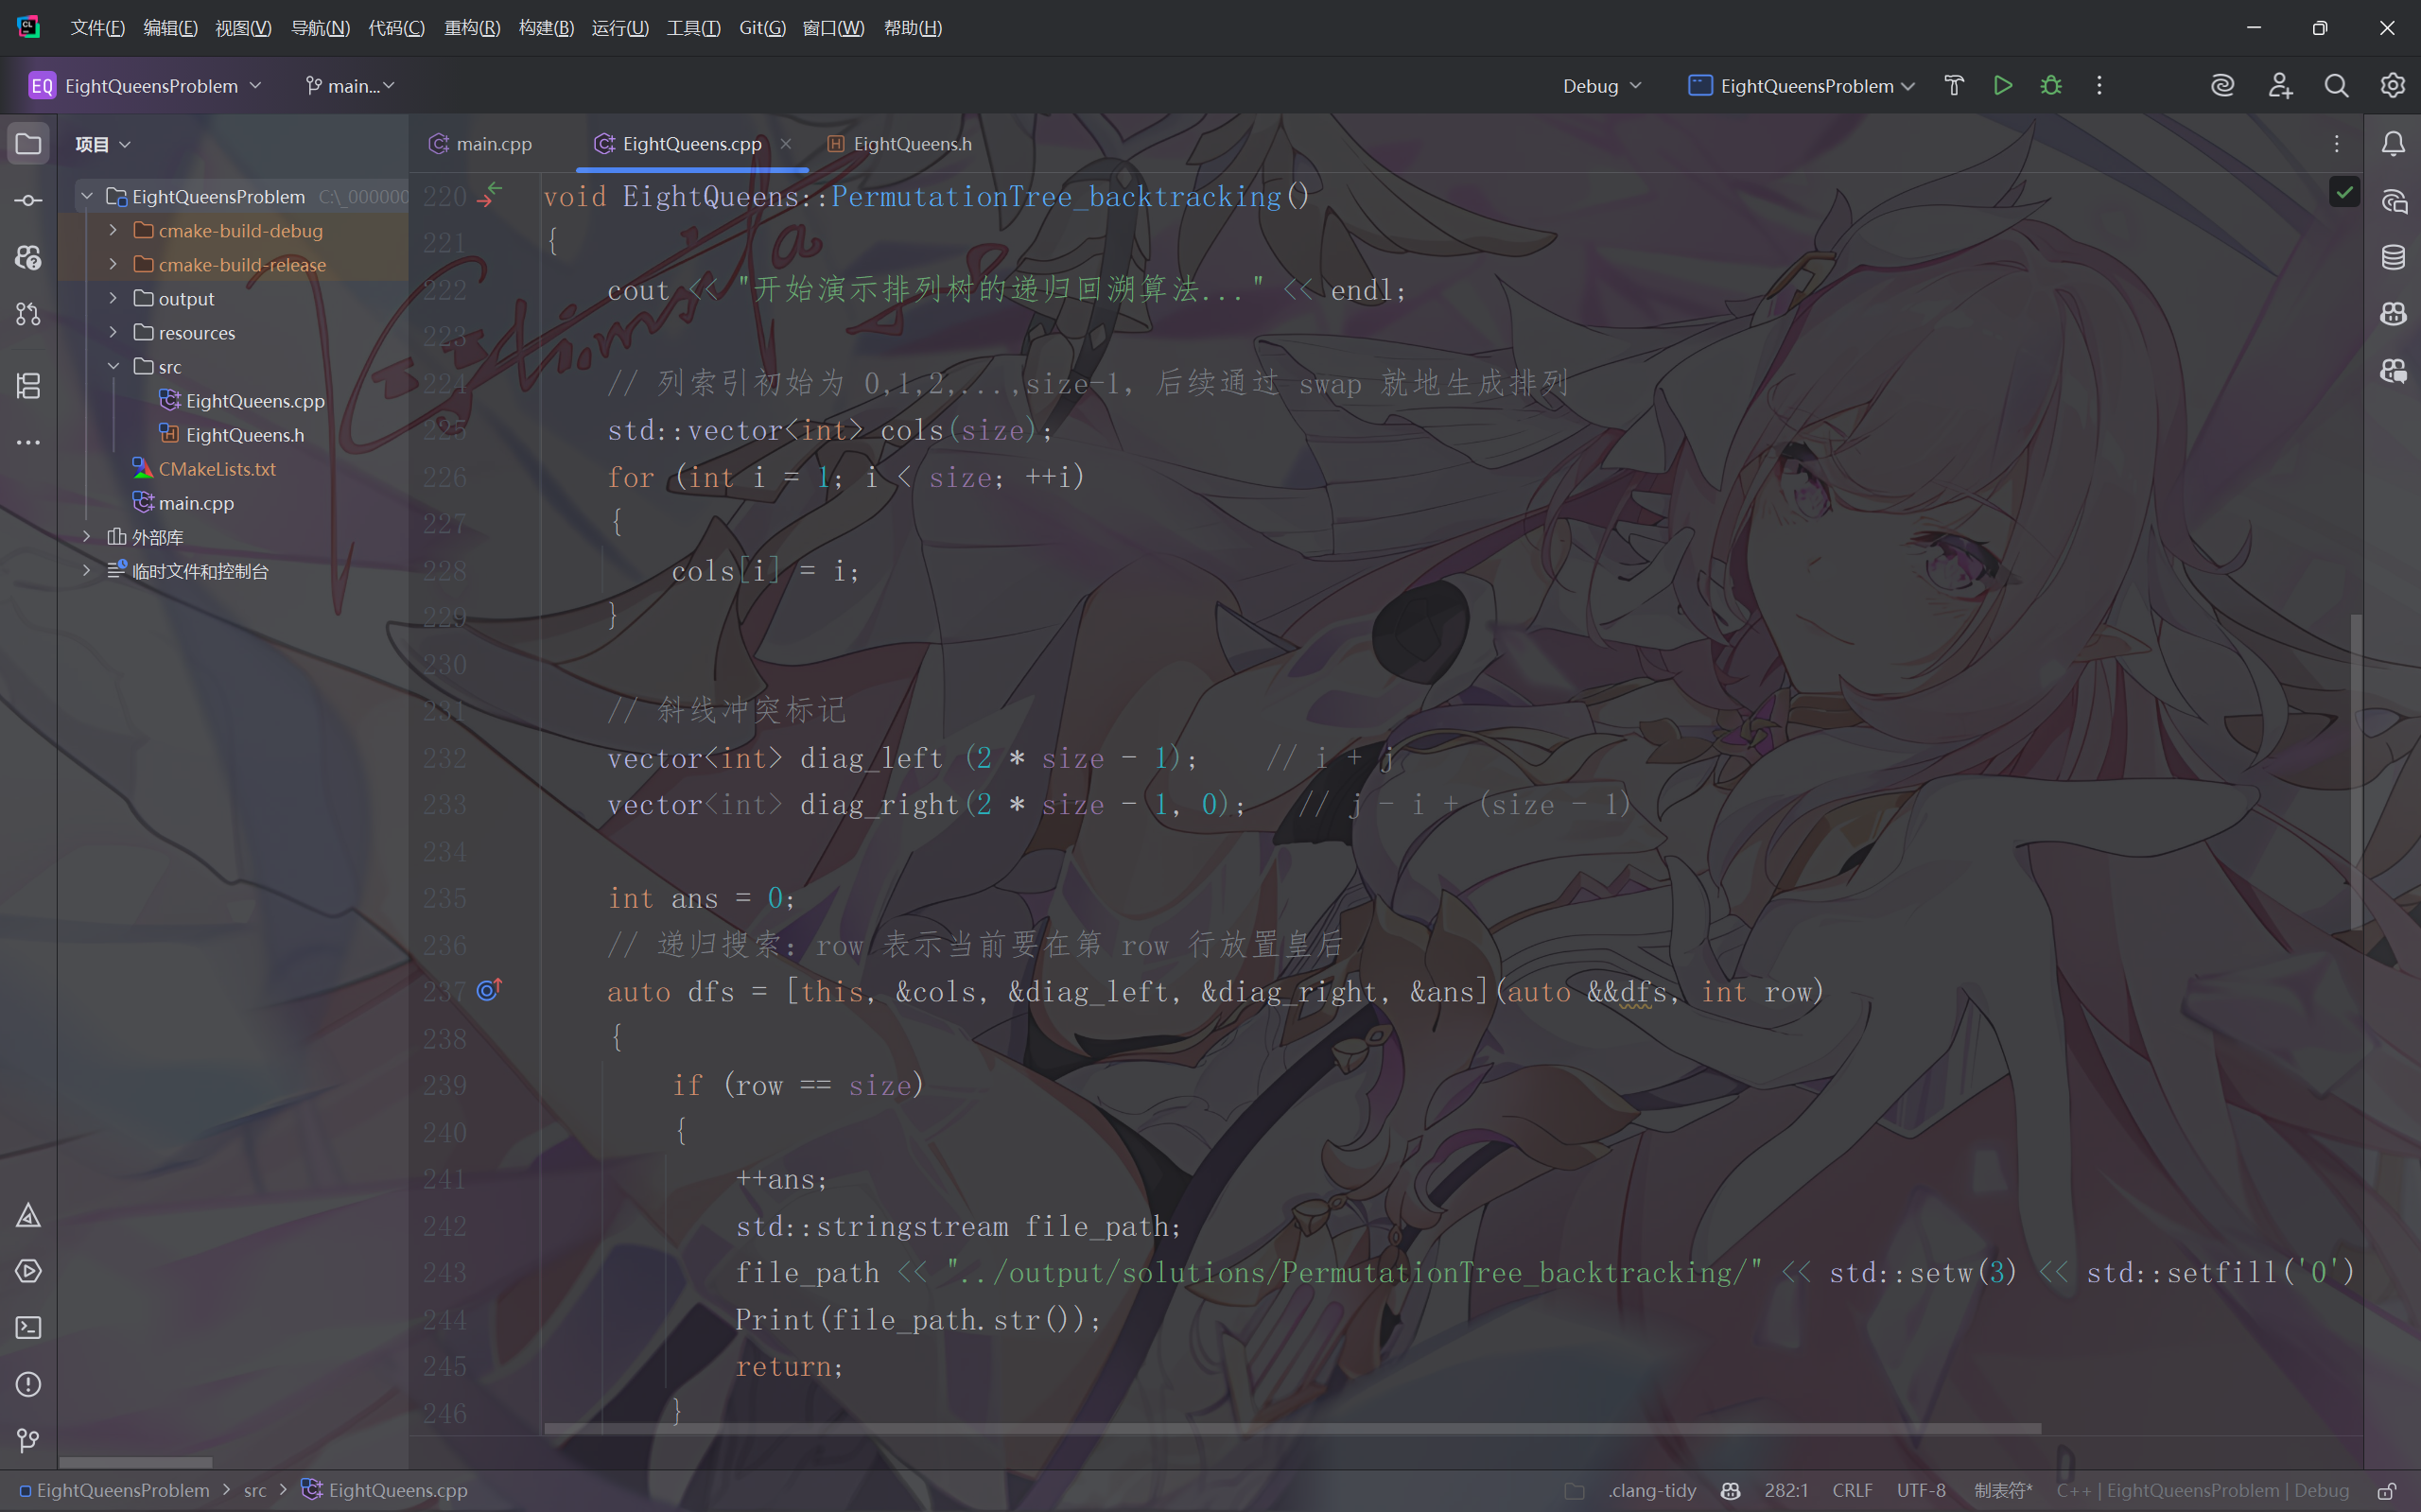
\includegraphics[width=\textwidth]{../images/排列树回溯代码1.png}\\[0.5em]
\captionof{figure}{排列树回溯代码1}
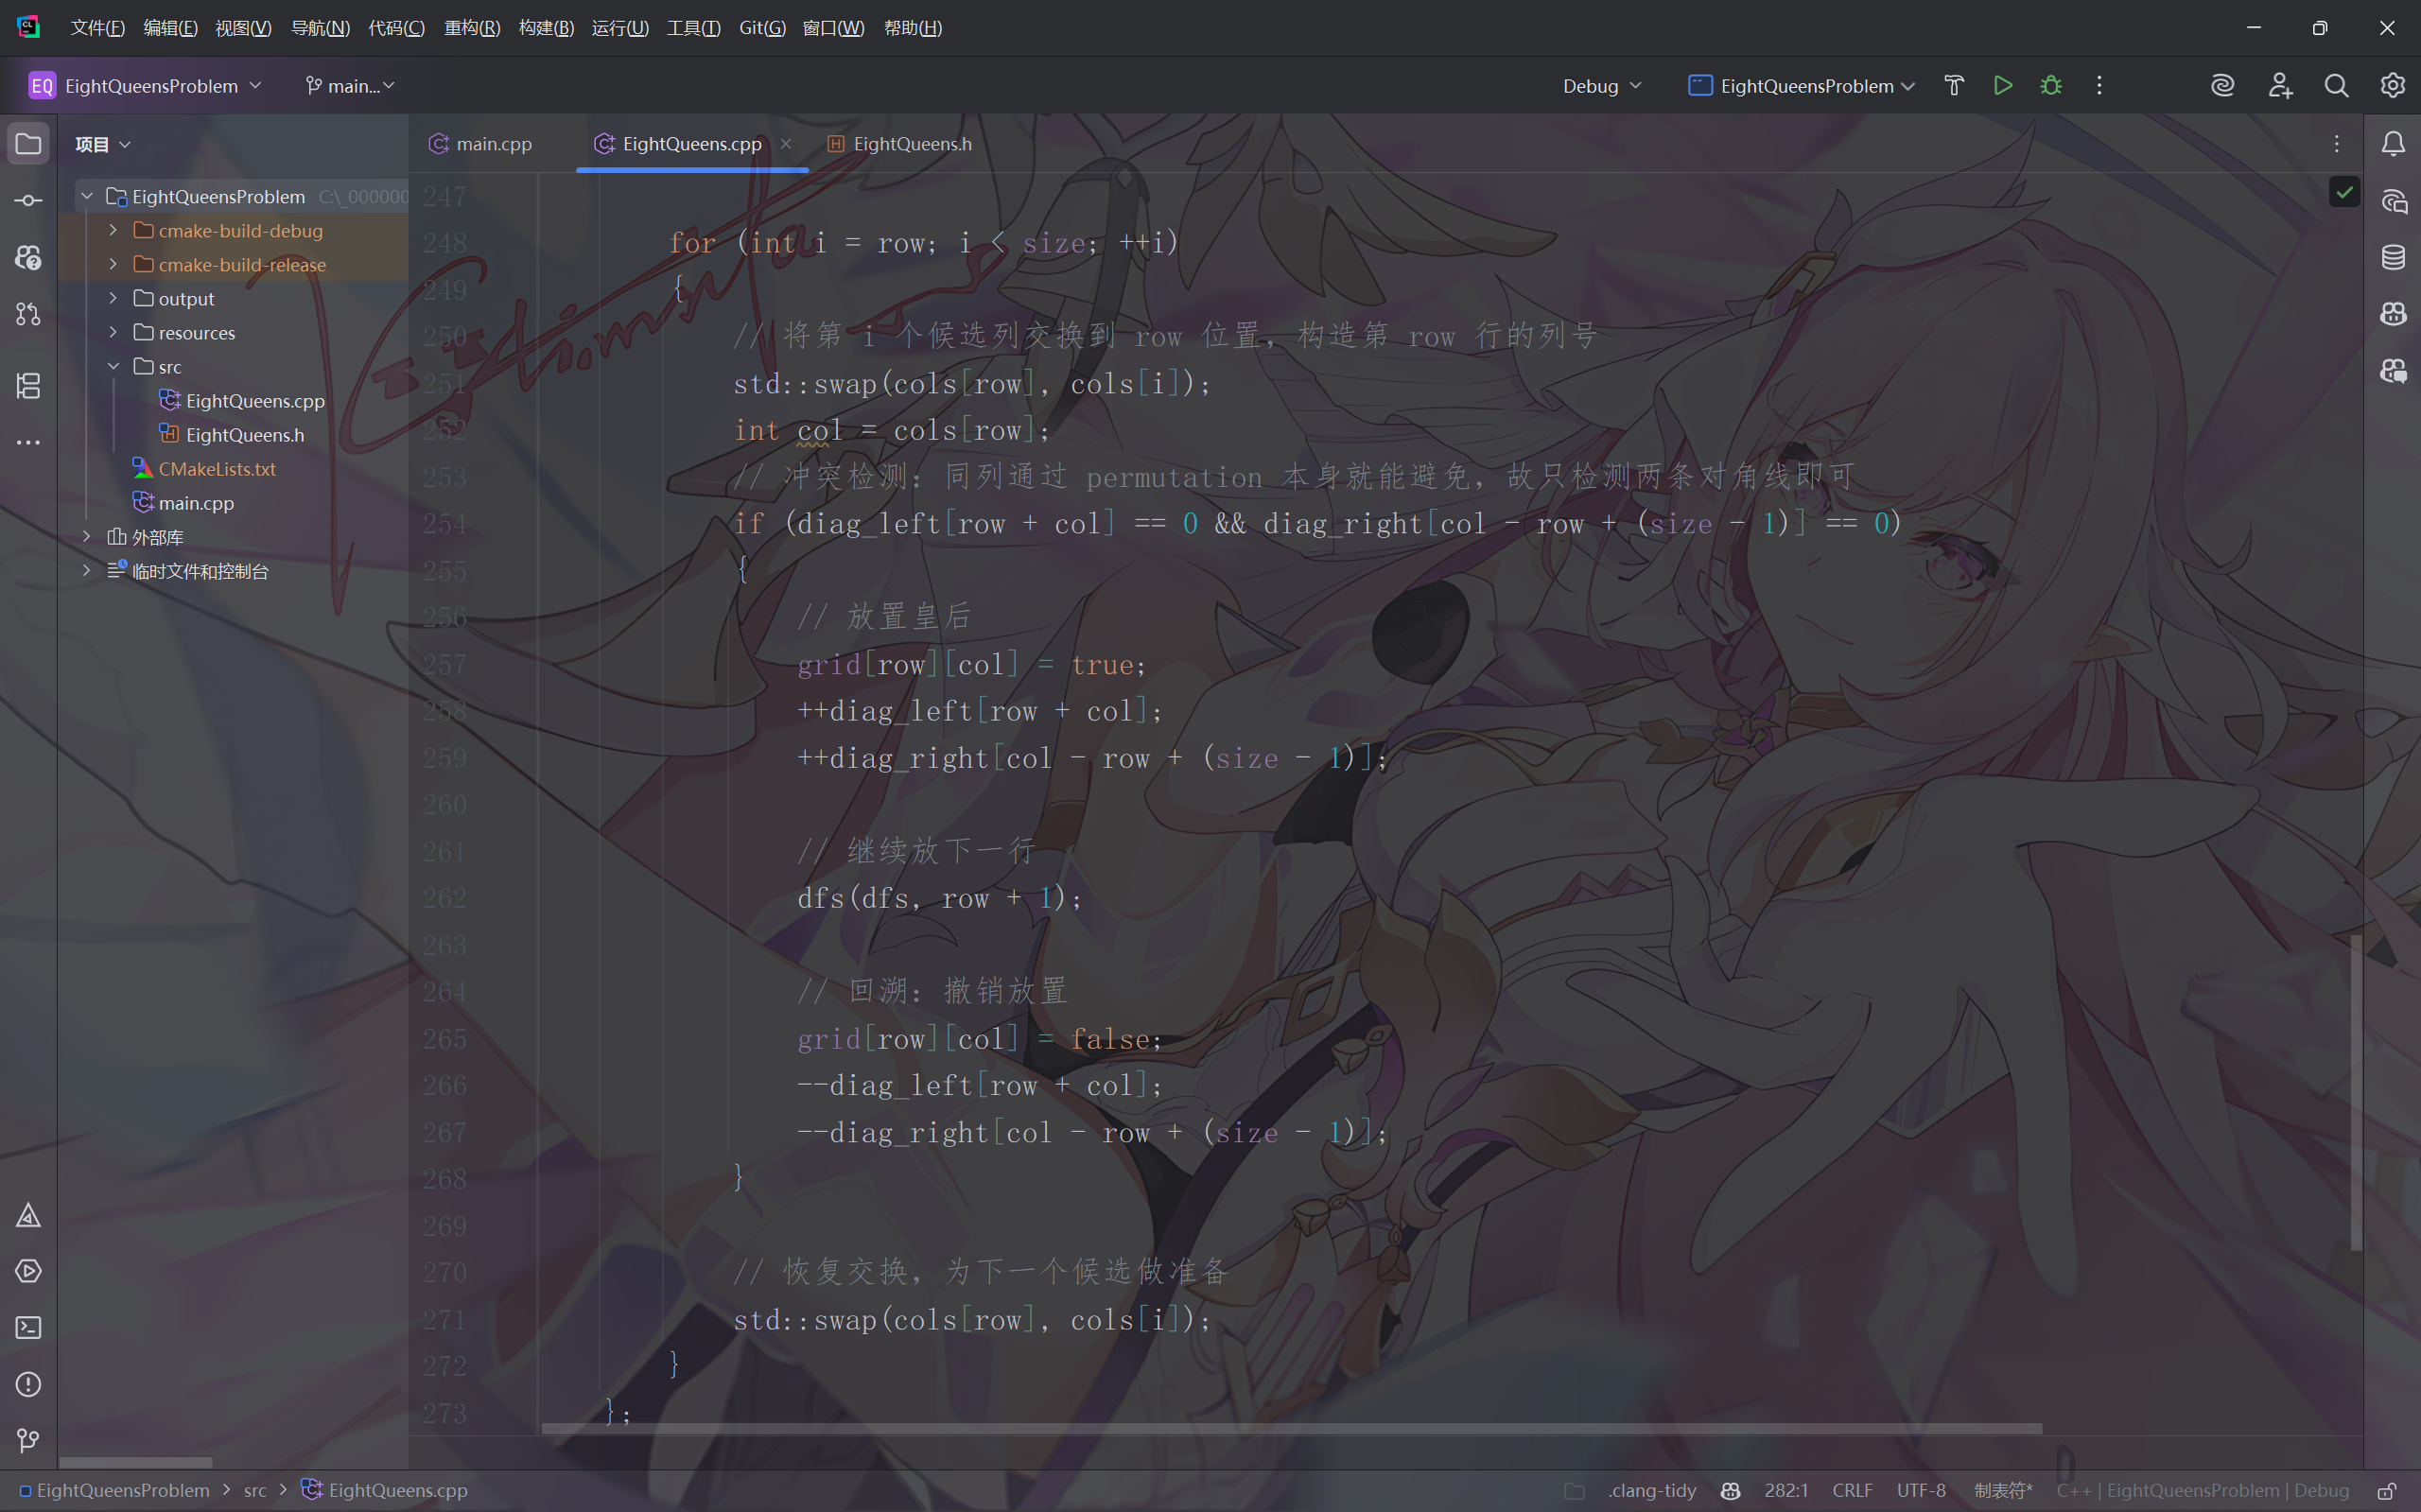
\includegraphics[width=\textwidth]{../images/排列树回溯代码2.png}\\[0.5em]
\captionof{figure}{排列树回溯代码2}
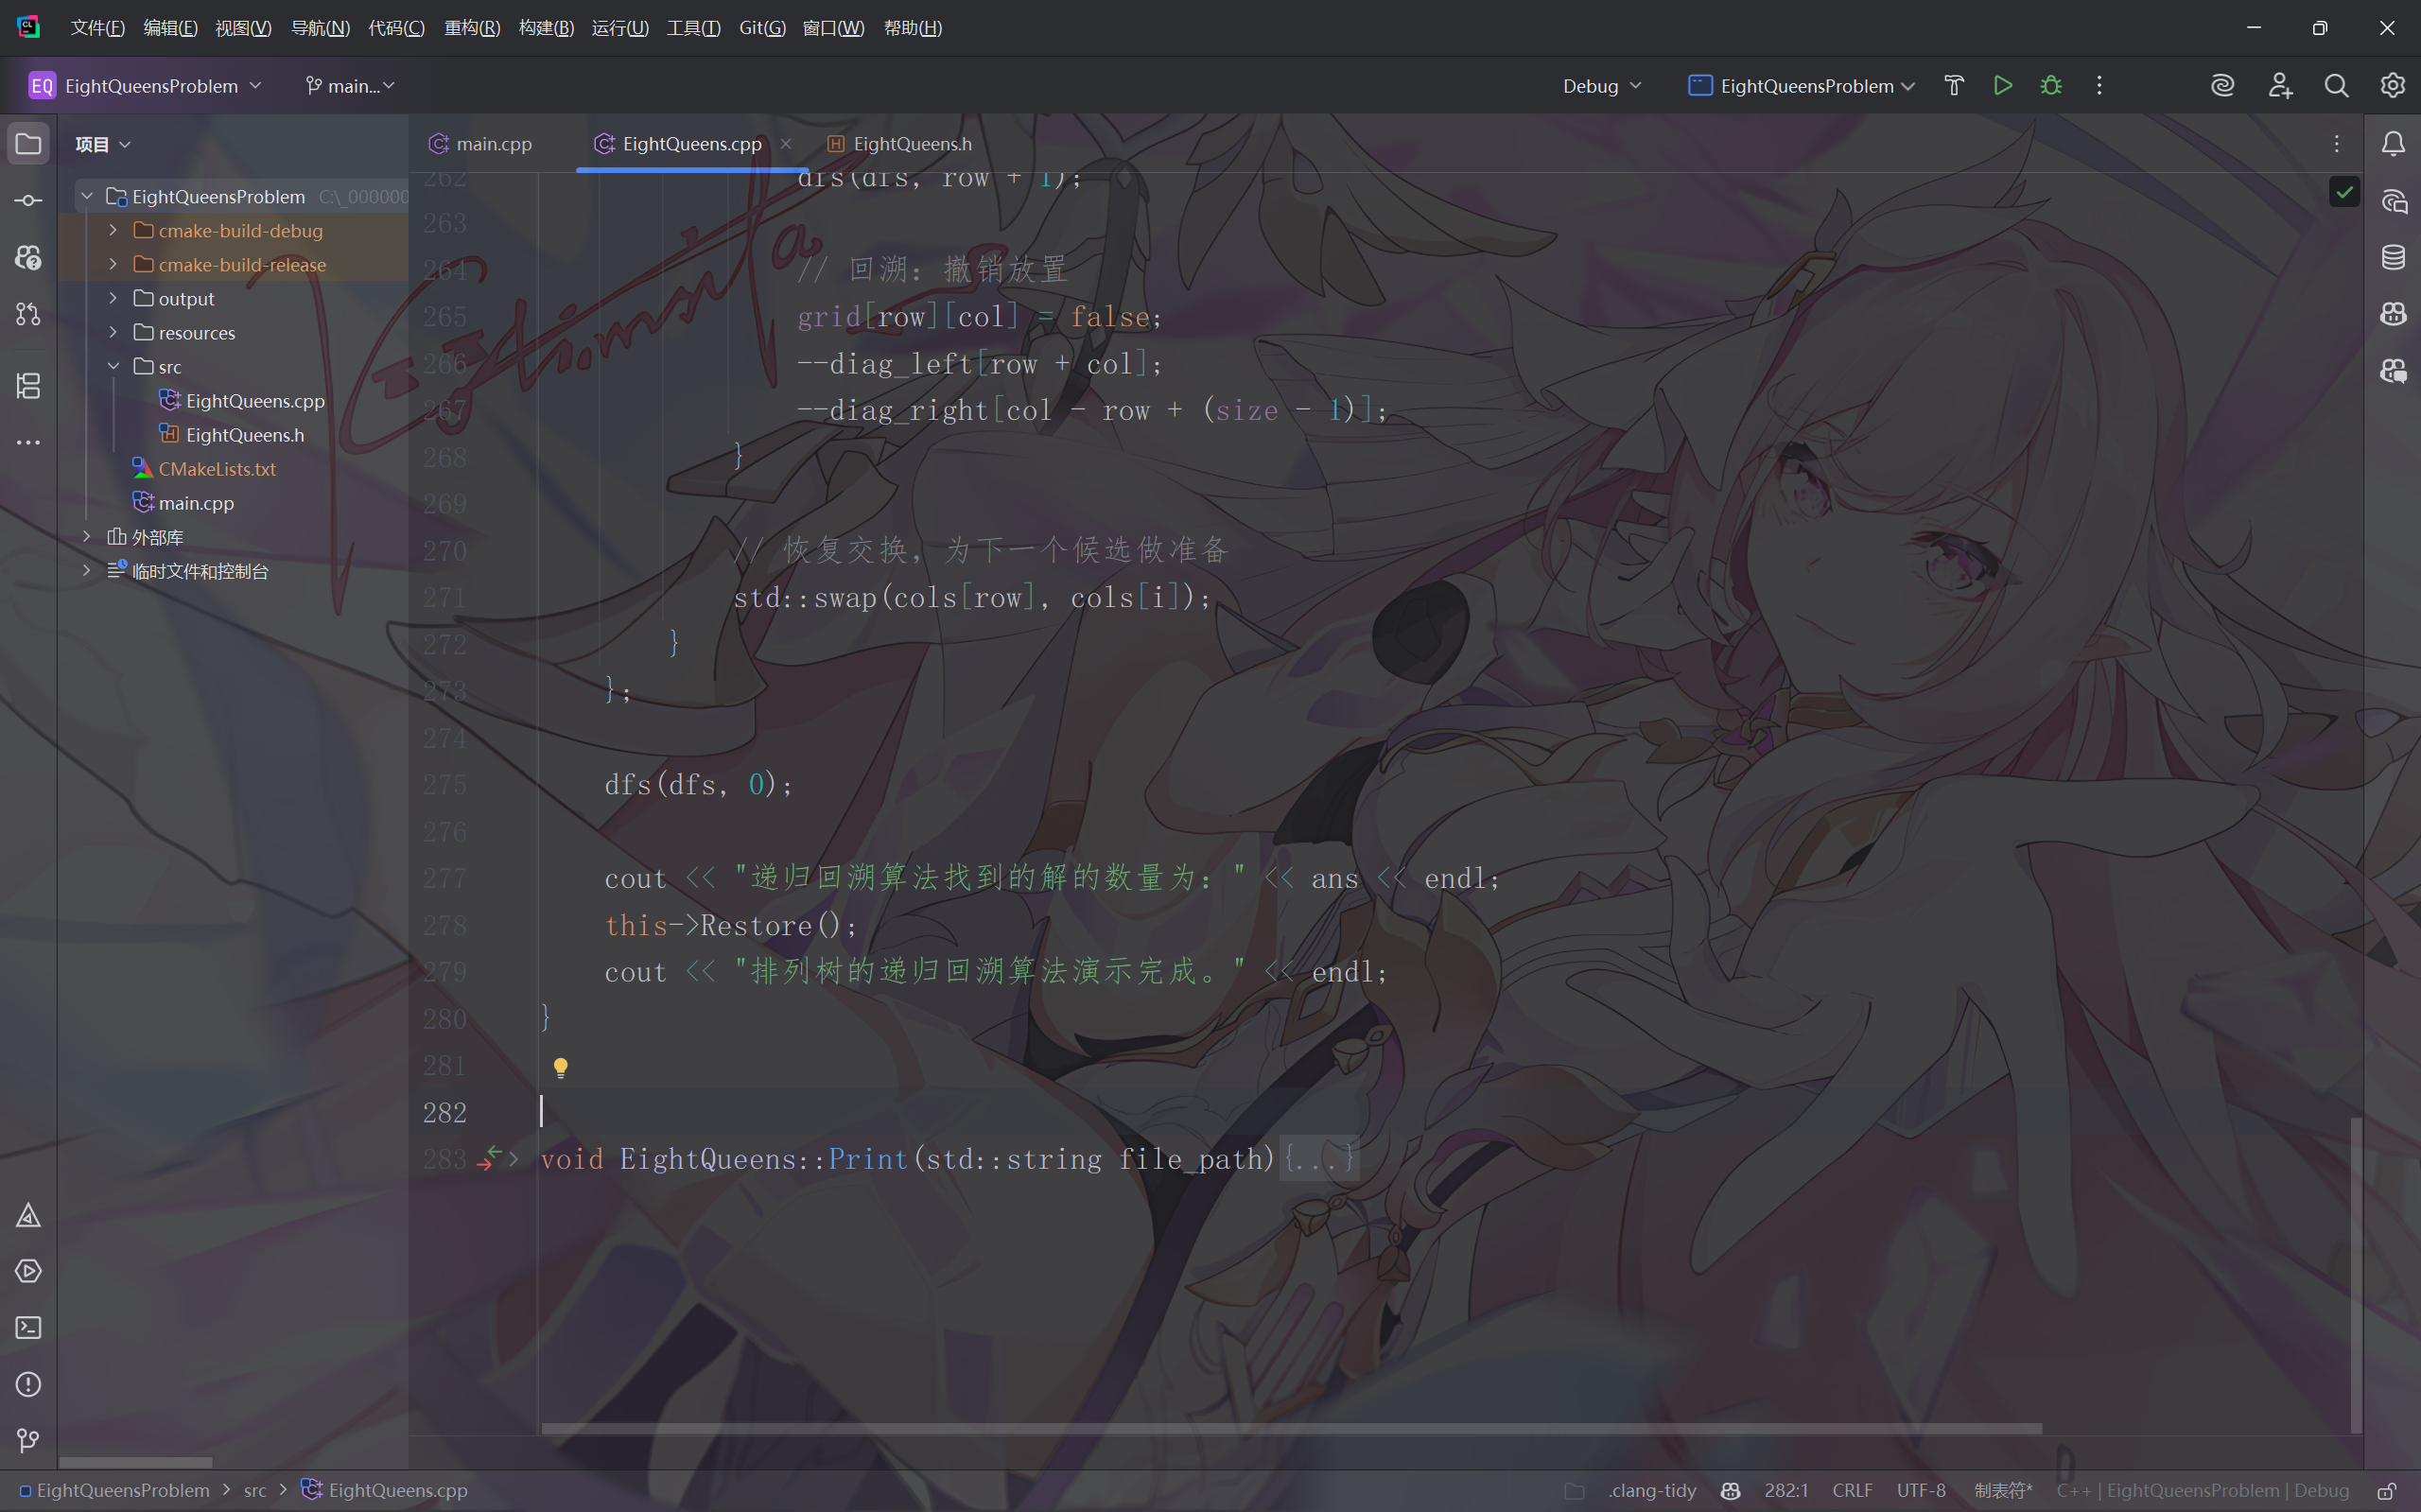
\includegraphics[width=\textwidth]{../images/排列树回溯代码3.png}\\[0.5em]
\captionof{figure}{排列树回溯代码3}

\section{实验结果与分析}

\subsection{实验结果}

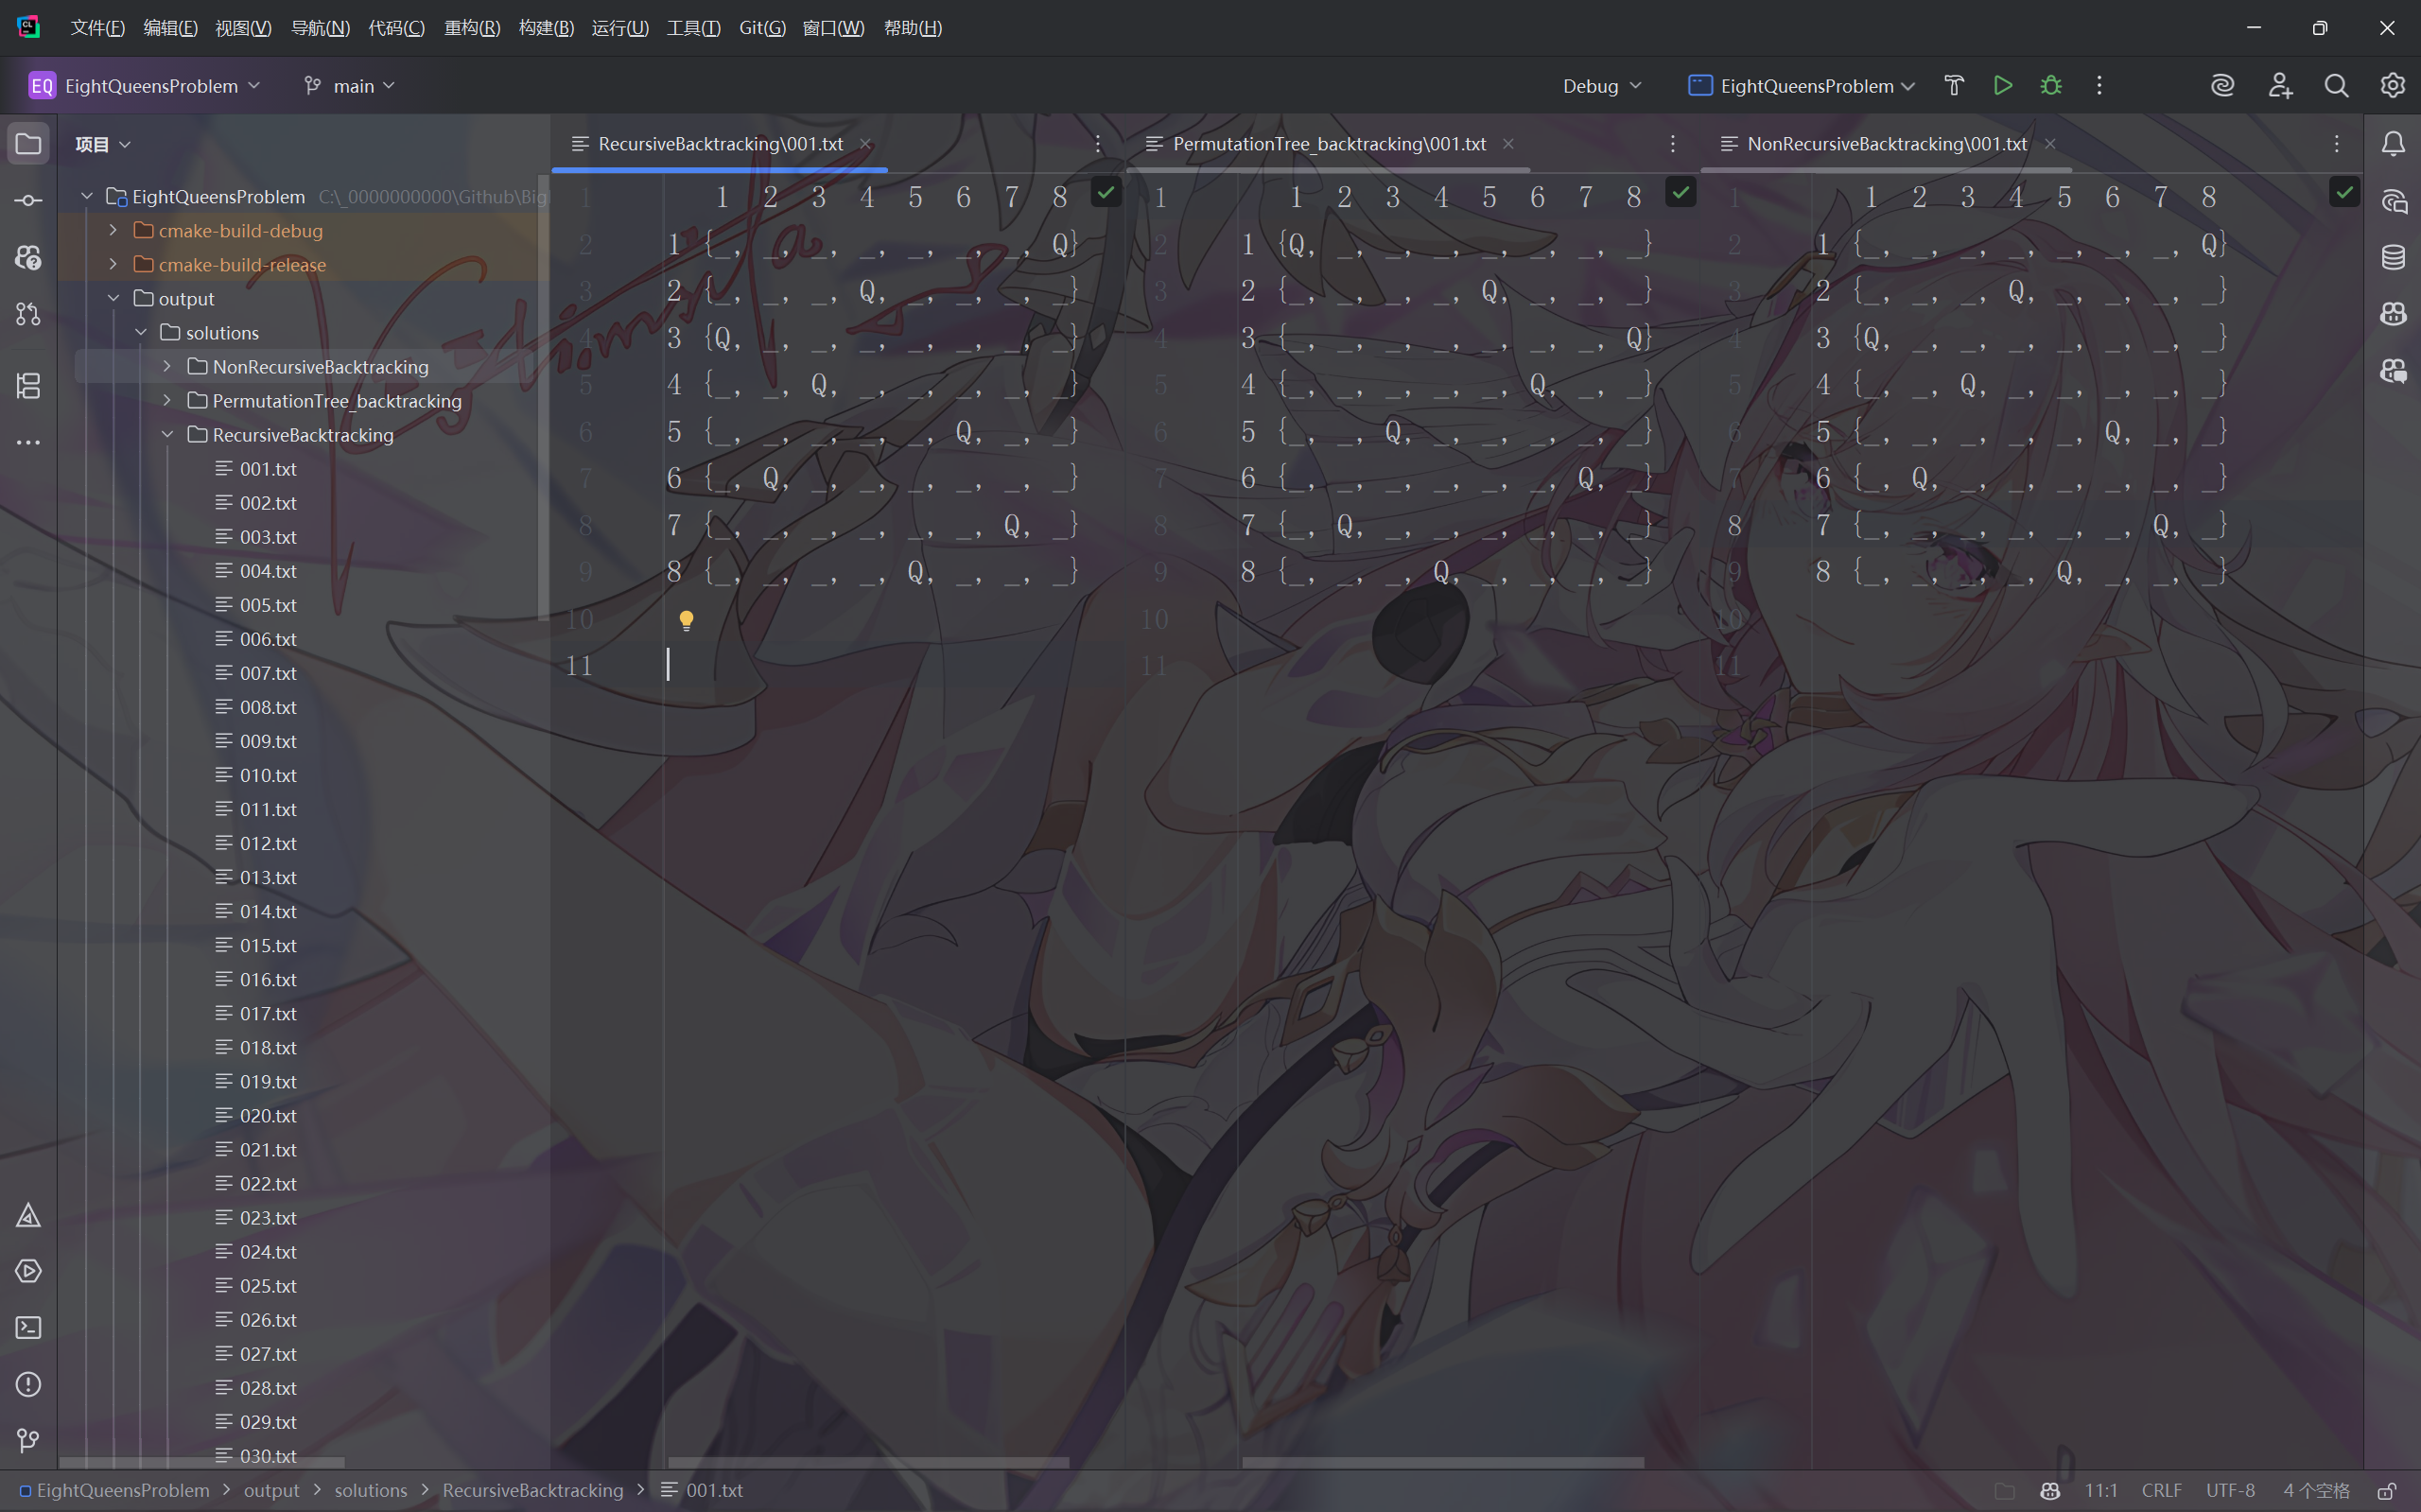
\includegraphics[width=\textwidth]{../images/实验结果.png}\\[0.5em]
\captionof{figure}{实验结果}

\subsection{算法效率分析}

\begin{table}[H]
\centering
\begin{tabular}{|c|c|c|c|}
\hline 
算法         & 解的数量 & 运行时间 & 特点分析                 \\ \hline
递归回溯法   & 92       & 28ms     & 实现简单,递归深度大     \\ \hline
非递归回溯法 & 92       & 64ms     & 避免递归开销,但效率很低 \\ \hline
排列树回溯法 & 92       & 16ms     & 生成全排列,效率高       \\ \hline
\end{tabular}
\end{table}

\section{实验代码}

\textbf{1. 进程主函数(main)}
\begin{lstlisting}[language=C++, breaklines=true]
int main()
{
	// 将控制台输出编码设置为 UTF-8,使得中文能正确输出
	SetConsoleOutputCP(CP_UTF8);
	// 将 C++ 与 C 的输入输出流解除同步
	std::ios::sync_with_stdio(false);

	// 创建八皇后问题的实例并调用菜单函数
	EightQueens eightQueens;
	eightQueens.Menu();

	return 0;
}
\end{lstlisting}

\textbf{2. 算法实现类(EightQueens)}
\begin{lstlisting}[language=C++, breaklines=true]
EightQueens::EightQueens() : size(8), grid(size, vector<bool>(size, false))
{}

void EightQueens::Menu()
{
	cout << "开始进行八皇后问题的求解算法演示..." << endl;
	cout << "[键入 Enter 键继续]" << endl;
	LINE_IGNORE

	// 不断读取用户输入,进行算法演示
	while (1)
	{
		cout << "请选择要演示的算法:" << endl;
		cout << "1. 递归回溯" << endl;
		cout << "2. 非递归回溯" << endl;
		cout << "3. 排列树的递归回溯" << endl;
		cout << "q. 退出" << endl;

		string choice;
		getline(cin, choice);
		if (choice == "1")
			Recursive_backtracking();
		else if (choice == "2")
			NonRecursive_backtracking();
		else if (choice == "3")
			PermutationTree_backtracking();
		else if (choice == "q")
			break;
		else
			cout << "无效的选择,请重新输入。" << endl;

		cout << "[键入 Enter 键继续]" << endl;
		LINE_IGNORE
	}
	cout << "程序已退出。" << endl;
}

void EightQueens::Restore()
{
	grid.assign(size, vector<bool>(size, false));
}

void EightQueens::Recursive_backtracking()
{
	cout << "开始进行递归回溯算法..." << endl;

	// 递归回溯算法的核心逻辑
	// 使用四个数组来记录每一行、每一列和两条对角线上当前放置的皇后数量
	vector<int> rows(size);
	vector<int> cols(size);
	vector<int> diag_left (2 * size - 1);
	vector<int> diag_right(2 * size - 1);
	int ans = 0; // 解的数量
	auto Dfs = [this, &rows, &cols, &diag_left, &diag_right, &ans](auto &&Dfs, int i, int j, int count_queen) -> void
	{

		// 如果所有格子都被判断过,结束递归搜索,返回答案
		if (i == size)
		{
			// 如果正好放置了八个皇后,解的数量加一
			if (count_queen == size)
			{
				++ans;
				// 打印当前棋盘到文件

				stringstream file_path; 
				file_path << "../output/solutions/RecursiveBacktracking/" << setw(3) << setfill('0') << ans << ".txt";
				Print(file_path.str());
			}
			return;
		}

		/*
		对于每个位置,分成放置皇后和不放置皇后两种情况进行递归求解
		*/

		// 如果当前位置不放置皇后,直接进入下一个位置
		j + 1 < size ? Dfs(Dfs, i, j + 1, count_queen) : Dfs(Dfs, i + 1, 0, count_queen);

		// 如果当前位置放置皇后,检查是否满足条件,满足条件则进入下一个位置
		if (rows[i] || cols[j] || diag_left[i + j] || diag_right[size - (i - j)])
			return;
		// 在棋盘上放置皇后,更新相关状态
		grid[i][j] = true;
		++rows[i];
		++cols[j];
		++diag_left[i + j];
		++diag_right[size - (i - j)];
		// 进入下一个位置
		j + 1 < size ? Dfs(Dfs, i, j + 1, count_queen + 1) : Dfs(Dfs, i + 1, 0, count_queen + 1);
		// 回溯,撤销放置皇后操作,恢复相关状态
		grid[i][j] = false;
		--rows[i];
		--cols[j];
		--diag_left[i + j];
		--diag_right[size - (i - j)];
	};
	// 执行递归回溯算法
	Dfs(Dfs, 0, 0, 0);

	// 输出结果
	cout << "递归回溯算法找到的解的数量为:" << ans << endl;

	// 算法演示完成后恢复棋盘
	this->Restore();
	cout << "递归回溯算法完成,所有可行解已被输出到文件。" << endl;
}

void EightQueens::NonRecursive_backtracking()
{
	// 正常人不会用这种垃圾算法……
	cout << "开始演示非递归回溯算法..." << endl;

	// 使用四个数组来记录每一行、每一列和两条对角线上当前放置的皇后数量
	vector<int> rows(size);
	vector<int> cols(size);
	vector<int> diag_left (2 * size - 1);
	vector<int> diag_right(2 * size - 1);

	struct Data 
	{
	    int i, j;        // 当前位置 (i,j)
	    int count;       // 到目前为止已放置的皇后数
	    int branch;      // 下一个要尝试的分支:0=跳过,1=放置,2=完成回退
	    bool placed;     // 本层是否放置过皇后,用于回退时恢复状态
	};

	int ans = 0;
	stack<Data> stk;
	stk.push({0, 0, 0, 0, false});
	while (!stk.empty())
	{
		auto &[i, j, count, branch, placed] = stk.top();
		if (i == size)
		{
			if (count == size)
			{
				++ans;
				stringstream file_path;
				file_path << "../output/solutions/NonRecursiveBacktracking/" << setw(3) << setfill('0') << ans << ".txt";
				Print(file_path.str());
			}
			stk.pop();
			continue;
		}
		// 计算下一个位置
		int next_i, next_j;
		j + 1 == size ?
			(next_i = i + 1, next_j = 0) :
			(next_i = i, next_j = j + 1);
		if (branch == 0)
		{
			// 分支 0:不在 (i,j) 放皇后,直接“递归”到下一个位置
			branch = 1;
			stk.push({next_i, next_j, count, 0, false});
		}
		else if (branch == 1)
		{
			// 分支 1:尝试在 (i,j) 放皇后
			branch = 2;
			if (rows[i] || cols[j] || diag_left[i + j]  ||diag_right[size - (i - j)])
				continue;
			// 放置皇后,更新状态
			grid[i][j] = true;
			++rows[i];
			++cols[j];
			++diag_left[i + j];
			++diag_right[size - (i - j)];
			placed = true;
			// 进入下一位置
			stk.push({next_i, next_j, count + 1, 0, false});
		}
		else
		{
			// 分支 2:两种尝试都结束,执行回退
			if (placed)
			{
				// 如果本层放过皇后,则撤销放置
				grid[i][j] = false;
				--rows[i];
				--cols[j];
				--diag_left[i + j];
				--diag_right[size - (i - j)];
			}
			stk.pop();
		}
	}

	cout << "非递归回溯算法找到的解的数量为:" << ans << endl;
	this->Restore();
	cout << "非递归回溯算法演示完成。" << endl;
}

void EightQueens::PermutationTree_backtracking()
{
    cout << "开始演示排列树的递归回溯算法..." << endl;

    // 列索引初始为 0,1,2,...,size-1,后续通过 swap 就地生成排列
    std::vector<int> cols(size);
    for (int i = 1; i < size; ++i)
	{
		cols[i] = i;
	}

    // 斜线冲突标记
    vector<int> diag_left (2 * size - 1);    // i + j
    vector<int> diag_right(2 * size - 1, 0);   // j - i + (size - 1)

    int ans = 0;
	// 递归搜索:row 表示当前要在第 row 行放置皇后
	auto dfs = [this, &cols, &diag_left, &diag_right, &ans](auto &&dfs, int row)
	{
		if (row == size)
		{
			++ans;
			std::stringstream file_path;
			file_path << "../output/solutions/PermutationTree_backtracking/" << std::setw(3) << std::setfill('0') << ans << ".txt";
			Print(file_path.str());
			return;
		}

		for (int i = row; i < size; ++i)
		{
			// 将第 i 个候选列交换到 row 位置,构造第 row 行的列号
			std::swap(cols[row], cols[i]);
			int col = cols[row];
			// 冲突检测:同列通过 permutation 本身就能避免,故只检测两条对角线即可
			if (diag_left[row + col] == 0 && diag_right[col - row + (size - 1)] == 0)
			{
				// 放置皇后
				grid[row][col] = true;
				++diag_left[row + col];
				++diag_right[col - row + (size - 1)];

				// 继续放下一行
				dfs(dfs, row + 1);

				// 回溯:撤销放置
				grid[row][col] = false;
				--diag_left[row + col];
				--diag_right[col - row + (size - 1)];
			}

			// 恢复交换,为下一个候选做准备
			std::swap(cols[row], cols[i]);
		}
	};

    dfs(dfs, 0);

    cout << "递归回溯算法找到的解的数量为:" << ans << endl;
    this->Restore();
    cout << "排列树的递归回溯算法演示完成。" << endl;
}

void EightQueens::Print(std::string file_path)
{
	// 创建文件目录
	create_directories(path(file_path).parent_path());
	// 打印当前棋盘到指定文件
	ofstream fout(file_path);
	
	fout << "   1  2  3  4  5  6  7  8" << endl;
	for (int i = 0; i < size; ++i)
	{
		auto &v = grid[i];
		fout << i + 1 << " {";
		for (int j = 0; j < size; ++j)
		{
			bool b = v[j];
			if (j != 0)
				fout << ", ";
			fout << (b ? "Q" : "_");
		}
		fout << "}" << endl;
	}
	fout << endl;
	fout.close();
}
\end{lstlisting}

\section{实验总结}
\begin{flushleft}
\songti\fontsize{16pt}{16pt}\selectfont
本次实验通过三种算法(递归回溯、非递归回溯和排列树回溯)实现了八皇后问题的求解,得到了 92 种同样的正确解果。

1. 递归回溯法实现简单,虽然递归深度较大,但整体运行效率较高。  

2. 非递归回溯法采用栈模拟递归,避免了函数调用开销,但整体效率特别低。 

3. 排列树回溯法通过全排列生成候选解,再进行斜线约束判断,实现了最高的效率。

实验结果表明,各算法均能正确输出所有解,并分别记录到指定的文件中。通过对比不仅验证了算法正确性,也为进一步优化提示了方向,例如改进递归边界条件和减少不必要的状态更新。本次实验对回溯法的理论和实现有了进一步深入的理解,同时也为后续复杂问题的求解奠定了良好基础。
\end{flushleft}

\end{document}